\documentclass[10pt, xcolor=x11names, compress]{beamer}
%\documentclass[10pt, xcolor=x11names, compress, handout]{beamer}
\usetheme{progressbar}
%\usecolortheme[named=Purple4]{structure}
\progressbaroptions{headline=sections,titlepage=normal,frametitle=normal}

\setbeamertemplate{navigation symbols}{}

\usepackage{iwona} 

\usepackage{alltt}
\usepackage{amsmath,amsfonts, amssymb, amscd}
\usepackage{hyperref}
\usepackage{setspace}
\usepackage{wasysym}
\usepackage{ulem}

\usepackage{calc}
\usepackage[overlay,absolute]{textpos}
\TPGrid[5mm,5mm]{20}{20}



\renewcommand{\Re}{\operatorname{Re}}
\renewcommand{\Im}{\operatorname{Im}}
\newcommand{\debye}{\operatorname{debye}}

\newcommand{\chik}{$\chi(k)$}
\newcommand{\chir}{$|\tilde{\chi}(R)|$}


\newcommand{\file}[1]{{\color{Firebrick4}\texttt{`#1'}}}
\newcommand{\multiple}{{\color{Orange3}\textsl{multiple}}}


\newcommand{\atoms}  {{\color{DarkOrchid4}\textsc{atoms}}}
\newcommand{\feff}   {{\color{DarkOrchid4}\textsc{feff}}}
\newcommand{\ifeffit}{{\color{DarkOrchid4}\textsc{ifeffit}}}
\newcommand{\athena} {{\color{DarkOrchid4}\textsc{athena}}}
\newcommand{\artemis}{{\color{DarkOrchid4}\textsc{artemis}}}

\renewenvironment<>{center}
{\begin{actionenv}#1\begin{originalcenter}}
{\end{originalcenter}\end{actionenv}}

\definecolor{guessp}   {rgb}{0.64,0.00,0.64}
\newcommand{\guessp}   {{\color{guessp}guess}}
\definecolor{defp}     {rgb}{0.00,0.55,0.00}
\newcommand{\defp}     {{\color{defp}def}}
\definecolor{setp}     {rgb}{0,0,0}
\newcommand{\setp}     {{\color{setp}set}}
\definecolor{lguessp}  {rgb}{0.24,0.11,0.56}
\newcommand{\lguessp}  {{\color{lguessp}lguess}}
\definecolor{skipp}    {rgb}{0.70,0.70,0.70}
\newcommand{\skipp}    {{\color{skipp}skip}}
\definecolor{restrainp}{rgb}{0.80,0.61,0.11}
\newcommand{\restrainp}{{\color{restrainp}restrain}}
\definecolor{afterp}   {rgb}{0.29,0.44,0.55}
\newcommand{\afterp}   {{\color{afterp}after}}
\definecolor{penaltyp} {rgb}{0.55,0.35,0.17}
\newcommand{\penaltyp} {{\color{penaltyp}penalty}}
\definecolor{mergep}   {rgb}{0.93,0.00,0.00}
\newcommand{\mergep}   {{\color{mergep}merge}}


\newcommand{\ybco}{YBa$_2$Cu$_3$O$_7$}
\newcommand{\eto}{EuTiO$_3$}
\newcommand{\bton}{BaTaO$_2$N}
\newcommand{\ufivemineral}%
{U$^{\mathrm{V}}$(H$_2$O)$_2$(U$^{\mathrm{VI}}$O$_2$)$_2$O$_4$(OH)+4$\cdot$H$_2$O}

\mode<presentation>

\title{Introduction to Inner Shell Spectroscopy}

\author{Bruce Ravel}
\institute[NIST]{Synchrotron Methods Group, Materials Measurement Science Division\\%
  Materials Measurement Laboratory\\%
  National Institute of Standards and Technology\\%
  \&\\%
  Local Contact, Beamline X23A2\\%
  National Synchrotron Light Source\\~}


%\date[Diamond2011]{EXAFS Data Analysis workshop 2011\\
  Diamond Light Source\\November 14--17, 2011\\~}

\date{SUNY Binghamton\\25 October 2012}

\begin{document}
\maketitle

\begin{frame}
  \frametitle{Copyright}
  \tiny

  This document is copyright \copyright 2007-2010 Bruce Ravel.

  \begin{center}
    
\includegraphics[width=1.0cm]{images/somerights20}
  \end{center}

  This work is licensed under the Creative Commons
  Attribution-ShareAlike License.  To view a copy of this license,
  visit \href{http://creativecommons.org/licenses/by-sa/3.0/}
  {\color{Purple4}\texttt{http://creativecommons.org/licenses/by-sa/3.0/}}
  or send a letter to Creative Commons, 559 Nathan Abbott Way,
  Stanford, California 94305, USA.

  \begin{description}
  \item[You are free:] %
    \begin{itemize}
    \item \textbf{to Share} --- to copy, distribute, and transmit the work
    \item \textbf{to Remix} --- to adapt the work
    \end{itemize}
  \item[Under the following conditions:] %
    \begin{itemize}
    \item Attribution. You must attribute the work in the manner
      specified by the author or licensor (but not in any way that
      suggests that they endorse you or your use of the work).
    \item Share Alike. If you alter, transform, or build upon this
      work, you may distribute the resulting work only under the same,
      similar or a compatible license.
    \item Any of these conditions can be waived if you get permission
      from the author.
    \end{itemize}
  \end{description}
  \begin{itemize}
  \item For any reuse or distribution, you must make clear to others
    the license terms of this work. The best way to do this is with a
    link to the URL for this document.
  \item Any of the above conditions can be waived if you get
    permission from the copyright holder.
  \item Nothing in this license impairs or restricts the author's
    moral rights.
  \end{itemize}

  Your fair dealing and other rights are in no way affected by the
  above.  This is a human-readable summary of the Legal Code (the full
  license).


\end{frame}

%%% Local Variables:
%%% mode: latex
%%% TeX-master: "pimst2"
%%% End:


\section[Introduction]{Introduction}

%\subsection{Beamline}
\begin{frame}
  \frametitle{This Talk}
  
  This talk is an introduction to the inner-shell spectroscopies, XAS
  and XRF.

  \bigskip

  \begin{block}{Outline}
    \begin{itemize}
    \item An overview of the basic physics of inner shell spectroscopies
    \item An introduction to XAS and XRF beamline instrumentation
    \item A flavor of the sorts of science that can be accomplished
      with XAS and XRF using examples from my own research.
    \end{itemize}
  \end{block}

  \bigskip

  My hope is that you will leave with a sense of how XAS and XRF might
  be applied to \alert{your} research.
\end{frame}

\setbeamercovered{dynamic}
%\setbeamercovered{transparent=50}
\begin{frame}
  \frametitle{XAS and XRF}

  \begin{center}
    \Large
    \alert{X}-ray \alert{A}bsorption \alert{S}pectroscopy\\
    and\\
    \alert{X}-\alert{R}ay \alert{F}luorescence spectroscopy\\[3ex]
    These are {\color{Firebrick4}inner shell}
    {\color{Purple4}spectroscopies}.
  \end{center}

  \begin{columns}[T]
    \begin{column}{0.5\linewidth}
      \uncover<2->{{\color{Firebrick4}Inner shell} means that an x-ray
        interacts primarily with a deep-core electron rather than with
        a valence electron.}
    \end{column}
    \begin{column}{0.5\linewidth}
      \uncover<3>{{\color{Purple4}Spectroscopy} means that some aspect
        of the interaction changes as a function of photon energy.}
    \end{column}
  \end{columns}
\end{frame}

\begin{frame}
  \frametitle{The basic physical process in XAS and XRF}

  \begin{center}
\only<beamer| beamer:1>{\includegraphics[width=0.7\linewidth]{images/atom.pdf}}%
\only<beamer| beamer:2>{\includegraphics[width=0.7\linewidth]{images/ion.pdf}}%
\only<beamer| beamer:3>{\includegraphics[width=0.7\linewidth]{images/emission.pdf}}
\only<beamer| beamer:4>{\includegraphics[width=0.7\linewidth]{images/auger.pdf}}
    \only<handout>{
      \includegraphics[width=0.25\linewidth]{images/atom.pdf}
      \includegraphics[width=0.25\linewidth]{images/ion.pdf}
      \includegraphics[width=0.25\linewidth]{images/emission.pdf}
      \includegraphics[width=0.25\linewidth]{images/auger.pdf}
    }
  \end{center}

  %\vskip -25pt

  \begin{enumerate}[<+->]
  \item An incoming photon interacts with a deep-core electron.  Shown
    here, a 1s electron is excited for a K-edge spectrum.
  \item The deep-core electron is promoted to some unoccupied state
    above the Fermi energy, propagates away, and leaves behind a
    core-hole.
  \item A short time later (1 or 2 femtoseconds), a higher-lying
    electron decays into the core-hole and emits a photon.
  \item Alternately, the energy from the higher-lying electron can be
    used to emit an Auger electron.
  \end{enumerate}
\end{frame}

\begin{frame}
  \frametitle{Characteristic energies}
  
  \small%
  Each element has a characteristic set of excitation and
  fluorescence energies.

  \medskip

  \begin{block}{}
    Iron: Z=26
  \end{block}
  \begin{columns}[T]
    \begin{column}{0.1\linewidth}
      ~
    \end{column}
    \begin{column}{0.3\linewidth}
      \begin{tabular}{cr}
        Edge &  Energy \\
        \hline
        \alert{K}    & \alert{7112}    \\
        L3   & 706.8   \\
        L2   & 719.9   \\
        L1   & 844.6
      \end{tabular}
    \end{column}
    \begin{column}{0.6\linewidth}
      \begin{tabular}{llcc}
        Line & Transition & Energy &  Strength \\
        \hline
        K$\alpha_1$ & \alert{K}-L3 & 6405.2 & 0.580\\
        K$\alpha_2$ & \alert{K}-L2 & 6392.1 & 0.294\\
        K$\beta_1$  & \alert{K}-M3 & 7059.3 & 0.082\\
        K$\beta_3$  & \alert{K}-M2 & 7059.3 & 0.043\\
        K$\beta_5$  & \alert{K}-M4,5 & 7110.0 & 0.001
      \end{tabular}
    \end{column}
  \end{columns}

  \begin{block}{}
    Uranium: Z=92
  \end{block}
  \begin{columns}[T]
    \begin{column}{0.1\linewidth}
      ~
    \end{column}
    \begin{column}{0.3\linewidth}
      \begin{tabular}{cr}
        Edge &  Energy \\
        \hline
        K    & 115606  \\
        \alert{L3}   & \alert{17166}   \\
        L2   & 20948   \\
        L1   & 21757
      \end{tabular}
    \end{column}
    \begin{column}{0.6\linewidth}
      \begin{tabular}{llcc}
        Line & Transition & Energy &  Strength \\
        \hline
        L$\alpha_1$ & \alert{L3}-M5   & 13614.0 & 0.686\\
        L$\alpha_2$ & \alert{L3}-M4   & 13438.0 & 0.077\\
        L$\beta_2$  & \alert{L3}-N4,5 & 16387.7 & 0.181\\
        L$\beta_5$  & \alert{L3}-O4,5 & 17063.2 & 0.038\\
        L$\beta_6$  & \alert{L3}-N1   & 15727.0 & 0.013\\
        L$_\ell$    & \alert{L3}-M1   & 11618.0 & 0.005\\
      \end{tabular}
    \end{column}
  \end{columns}
\end{frame}


\section[XAS]{X-ray Absorption}
\begin{frame}
  \frametitle<1| handout:1>{A simple picture of X-ray absorption} 
  \frametitle<2| handout:2>{X-ray absorption in condensed matter}

  \begin{overlayarea}{\linewidth}{6ex}
    \only<1| handout:1>{An incident x-ray of energy $E$ is absorbed,
      destroying a core electron of binding energy $E_0$ and emitting
      a photo-electron with kinetic energy $(E-E_0)$. The core state
      is eventually filled, ejecting a fluorescent x-ray or an Auger
      electron.  }%
    \only<2| handout:2>{The ejected photo-electron can scatter from
      neighboring atoms. $R$ has some relationship to $\lambda$ and
      there is a phase shift associated with the scattering event.
      Thus the outgoing and scattered waves interfere.  }%
  \end{overlayarea}

  \vskip 20pt

  \begin{columns}[T]
    \begin{column}{0.5\linewidth}
      \only<1| handout:1>{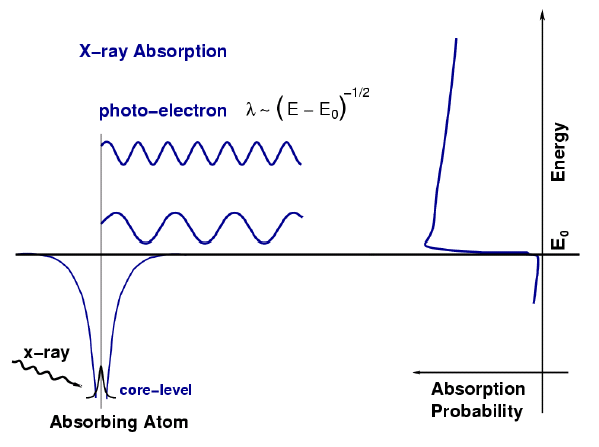
\includegraphics[width=\linewidth]{bare_atom.png}}
      \only<2| handout:2>{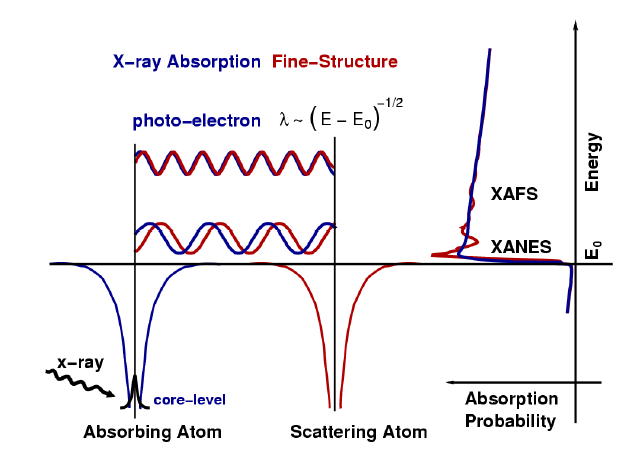
\includegraphics[width=\linewidth]{with_scattering.png}}
    \end{column}
    \begin{column}{0.5\linewidth}
      \begin{center}
        \only<1| handout:1>{
          An empty final state is required.\\
          {\alert{No available state, \\
              no absorption!}}\\
          When the incident x-ray energy is larger than the binding
          energy, there is a sharp increase in absorption.
        }
        \only<2| handout:2>{
          The scattering of the photo-electron wave function interferes
          with itself.\\[4ex]
          $\mu(E)$ depends on the density of states with energy
          $(E-E_0)$ at the absorbing atom.
        }
      \end{center}
    \end{column}
  \end{columns}

  \vskip 20pt

  \begin{overlayarea}{\linewidth}{3ex}
    \only<1| handout:1>{For an isolated atom, $\mu(E)$ has a sharp step at the
      core-level binding energy and is a smooth function of energy
      above the edge.}%
    \only<2| handout:2>{This interference \alert{at the absorbing atom} will vary
      with energy, causing the oscillations in $\mu(E)$.
    }%
  \end{overlayarea}
  \begin{bottomnote}[0.7][20] 
    Image from Matt Newville
  \end{bottomnote}
\end{frame}


\begin{frame}
  \frametitle{XAS and Valence State}

  \begin{columns}
    \begin{column}{0.5\linewidth}
      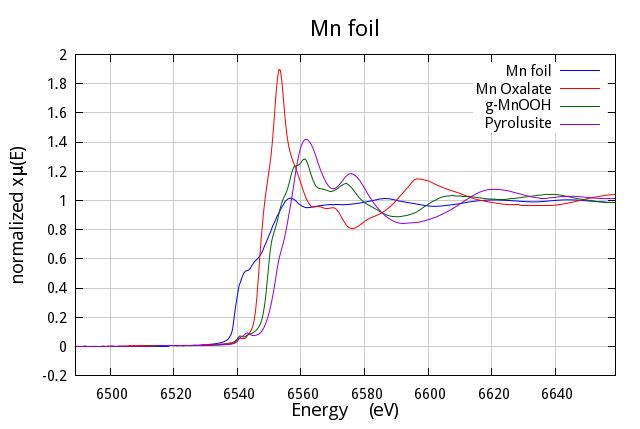
\includegraphics[width=\linewidth]{xas/mn_xanes.png}
    \end{column}
    \begin{column}{0.5\linewidth}
      As the valence increases\\[1ex]

      {\color{Blue3}Mn$^0$}$\rightarrow$ 
      \alert{Mn$^{2+}$} $\rightarrow$
      {\color{Green4}Mn$^{3+}$} $\rightarrow$
      {\color{Purple3}Mn$^{4+}$}\\[1ex]

      the edge position shifts to higher energy.
    \end{column}
  \end{columns}    

  \bigskip

  \begin{block}{XAS is a direct measure of valence state}
    \begin{itemize}
    \item Since each element has its own edge energy, an element's
      valence can be measured even in a heterogeneous sample
    \item Since x-rays are deeply penetrating into matter, minimal
      sample preparation is required
    \item No assumption of symmetry or periodicity is made, so the
      sample can be crystalline, amorphous, thin film, in solution,
      surface sorbed, $\cdots$ , \textit{whatever}
    \end{itemize}
  \end{block}

\end{frame}


\begin{frame}
  \frametitle{XAS and Local Atomic Structure}
  \begin{columns}[T]
    \begin{column}{0.34\linewidth}
      \visible<1->{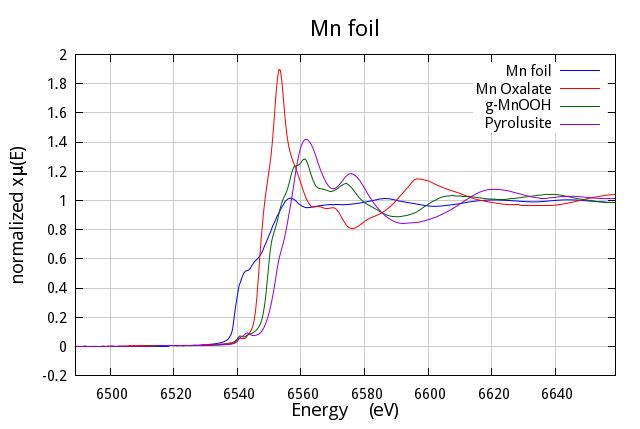
\includegraphics[width=\linewidth]{xas/mn_xanes}}

      \visible<2->{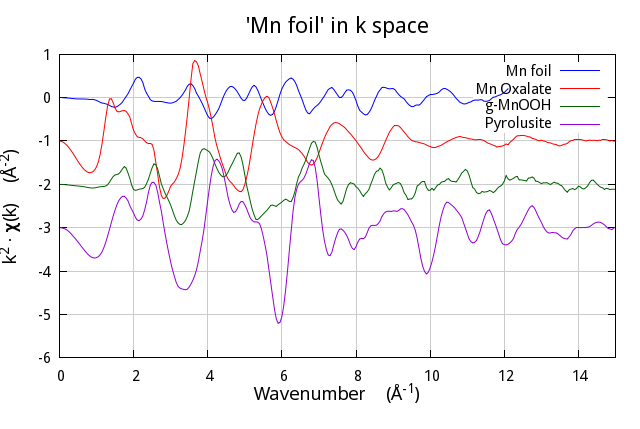
\includegraphics[width=\linewidth]{xas/mn_chik}}

      \visible<3>{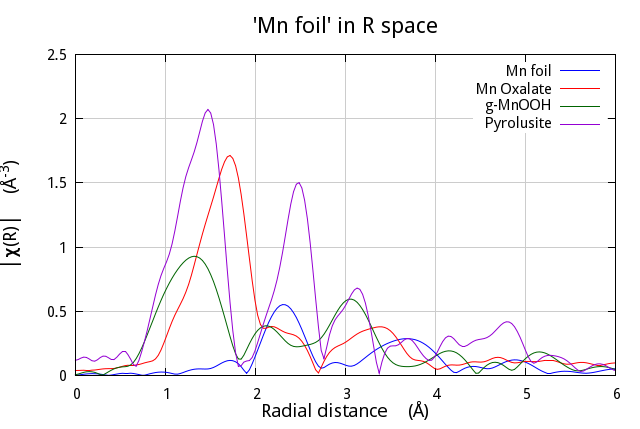
\includegraphics[width=\linewidth]{xas/mn_chir}}
    \end{column}
    \begin{column}{0.66\linewidth}
      \begin{itemize}[<+->]
      \item The different Mn species display big differences in the
        fine structure beyond the edge as the valence increases
        ({\color{Blue3}Mn$^0$}, \alert{Mn$^{2+}$},
        {\color{Green4}Mn$^{3+}$}, {\color{Purple3}Mn$^{4+}$}).  The
        white line and subsequent oscillations are quite
        different.\\[6ex]
      \item The oscillatory portion of the spectrum can be isolated
        and ...\\[6ex]
      \item ... Fourier transformed.  This FT function can be
        interpreted to yield partial pair distribution functions of
        atoms about the absorber.  The Mn-O distances are different
        for the \alert{Mn$^{2+}$}, {\color{Green4}Mn$^{3+}$}, and
        {\color{Purple3}Mn$^{4+}$} and clearly different from the
        Mn-Mn distance in {\color{Blue3}Mn metal}.
      \end{itemize}
    \end{column}
  \end{columns}
\end{frame}


\begin{frame}
  \frametitle{XAS is a direct measure of local structure}

  \begin{itemize}
  \item Since each element has its own edge energy, an element's
    local structure can be measured even in a heterogeneous sample
  \item Since x-rays are deeply penetrating into matter, minimal
    sample preparation is required
  \item No assumption of symmetry or periodicity is made, so the
    sample can be crystalline, amorphous, thin film, in solution,
    surface sorbed, $\cdots$ , \textit{whatever}
  \item Samples can be measured \textit{in situ}, which can mean
    \begin{itemize}
    \item cryostat or furnace
    \item high pressure cell
    \item electrochemistry cell or fuel cell
    \item peristaltic or stop-flow pump with liquid samples
    \item high field magnet
    \item etc...
    \end{itemize}
  \end{itemize}

  \begin{exampleblock}{}
    \begin{center}
      As a result, XAS is used in a very broad array of scientific
      disciplines
    \end{center}
  \end{exampleblock}


\end{frame}


\section[XRF]{X-ray Fluorescence}
\begin{frame}
  \frametitle{Fluorescence from Many Elements}
  X-ray fluorescence is a {\color{Purple4}spectroscopy} in which the
  incident energy is fixed and the energy dependence of the secondary
  photons is measured.

  \bigskip

  Every element with an edge \alert{below} the incident
  energy will fluoresce.

  \begin{center}
    Glass with every 2$^{\mathrm{nd}}$ element Ca--Ge, incident energy = 11153\,eV\\
    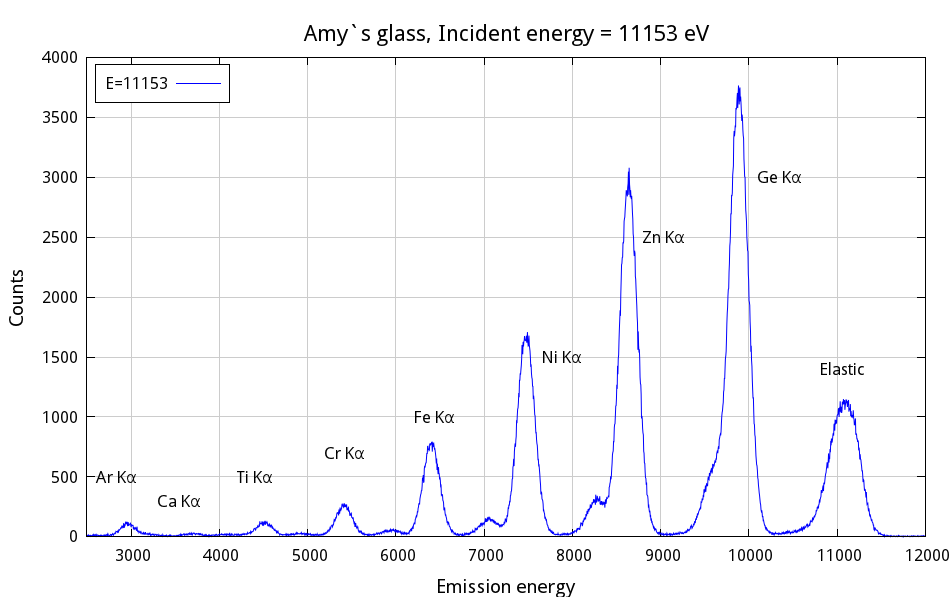
\includegraphics[width=0.75\linewidth]{xrf/glass_linear.png}
  \end{center}
  % \begin{center}
  %   NIST X-ray Fluorescence Standard \#1833, incident energy $\approx$ 12\,keV
  %   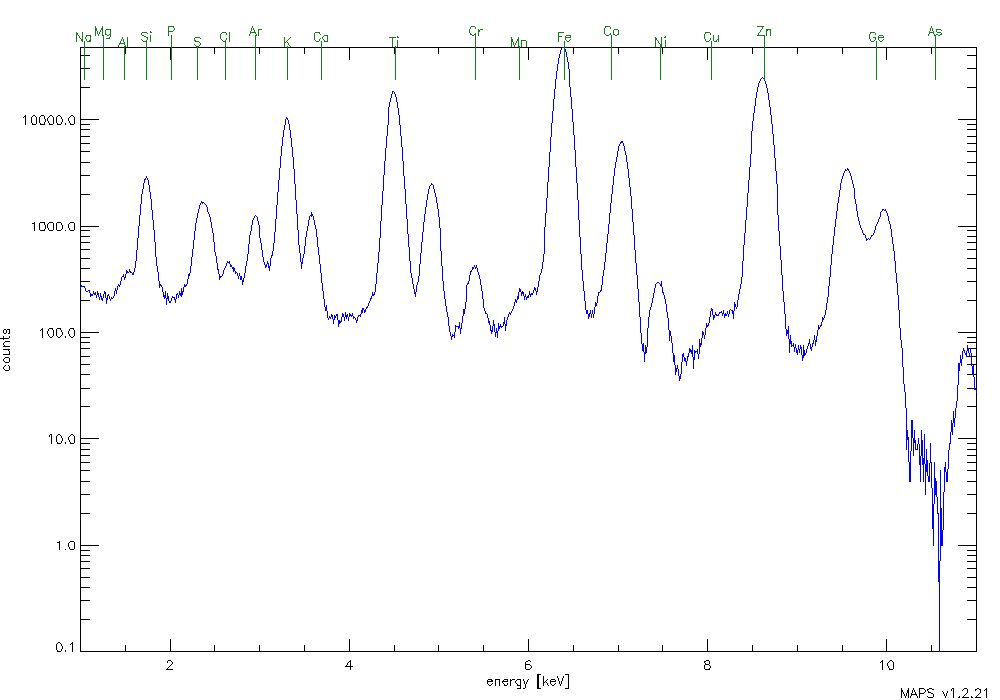
\includegraphics[width=0.7\linewidth]{xrf/NBS1833.png}
  % \end{center}

\end{frame}

\begin{frame}
  \frametitle{Fluorescence from A Sediment Sample}
  \begin{center}
    Here are the XRF spectra with incident beams \alert{above} and
    {\color{Blue4}below} the U L$_{III}$ edge for sediment heavily
    contaminated with uranium.

    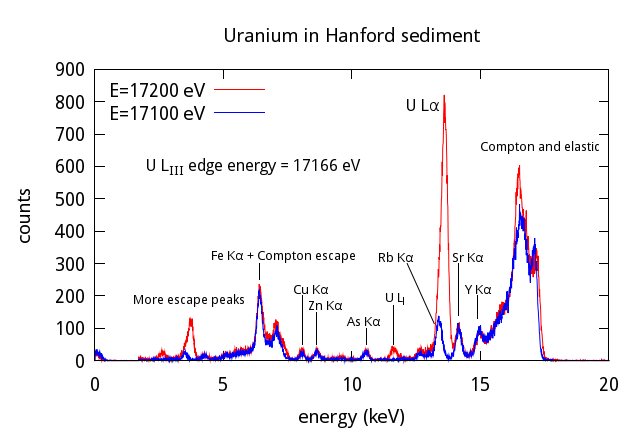
\includegraphics[width=0.7\linewidth]{xrf/xrf.png}
  \end{center}

  \begin{exampleblock}{}
    \begin{center}
      Combined with a standard measured under identical conditions,
      concentrations can be quantified.
    \end{center}
  \end{exampleblock}
\end{frame}
\begin{frame}
  \frametitle{Using the Fluorescence Spectrum for XAS}
  \begin{center}
    We can place a \alert{region of interest} (ROI) around the U
    L$\alpha$ peak and measure its variation as a function of incident
    energy.

    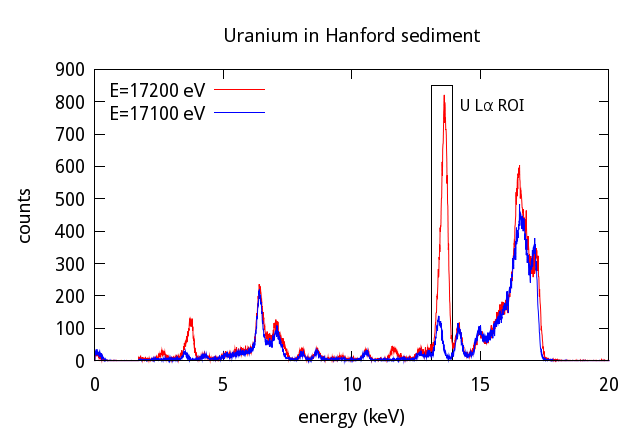
\includegraphics[width=0.7\linewidth]{xrf/roi.png}
  \end{center}

  \begin{exampleblock}{}
    \begin{center}
      In this way, we measure signal only from the absorber and reject
      all other photons entering the detector.
    \end{center}
  \end{exampleblock}
\end{frame}

\begin{frame}
  \frametitle{Learning About Your Sample}
  I once performed a study to measure the bonding between Hg and
  catalytic DNA molecules.  I was given a solution with
  \begin{columns}[T]
    \begin{column}{0.125\linewidth}
      ~
    \end{column}
    \begin{column}{0.3\linewidth}
      \begin{itemize}
      \item 3\,mM Hg chlorate
      \item 3\,mM DNA
      \end{itemize}
    \end{column}
    \begin{column}{0.45\linewidth}
      \begin{itemize}
      \item 50\,mM cacodylic acid (buffer)
      \item 100\,mM NaClO$_4$ (salt)
      \end{itemize}
    \end{column}
    \begin{column}{0.125\linewidth}
      ~
    \end{column}
  \end{columns}

  \medskip

  Here is the fluorescence spectrum:\\[1ex]
  \begin{columns}
    \begin{column}{0.5\linewidth}
      \visible<1->{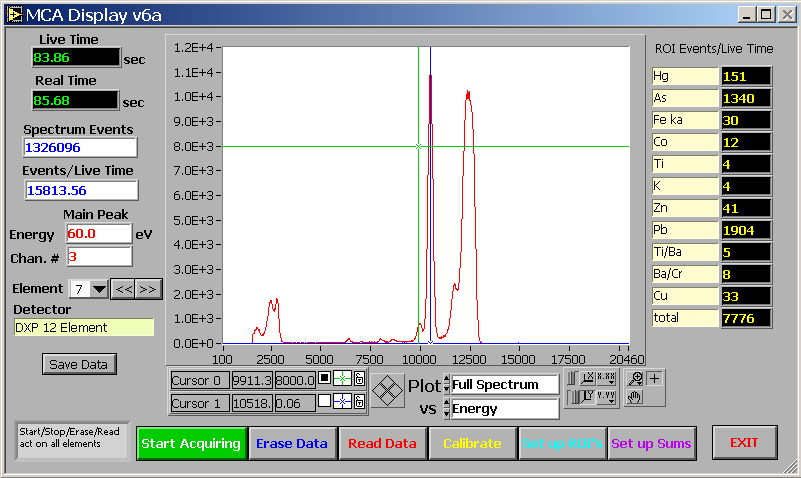
\includegraphics[width=\linewidth]{images/spectrum.png}}
    \end{column}
    \begin{column}{0.5\linewidth}
      \begin{center}
        \visible<2>{
          A quick Wikipedia search told me that cacodylic acid is:

          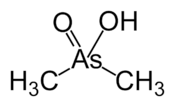
\includegraphics[width=0.35\linewidth]{images/cacodylate.png}

          \small
          The big peak is As K$\alpha$ ($\sim$10.5\,keV), the little one is
          Hg L$\alpha$ ($\sim$10\,keV).
        }
      \end{center}
    \end{column}
  \end{columns}
  \begin{textblock*}{0.5\linewidth}(0pt,19\TPVertModule)%
    \tiny%
    B.\ Ravel, et al., \textit{EXAFS studies of catalytic DNA sensors
      for mercury contamination of water}, Radiation Physics and
    Chemistry \textbf{78}:10 (2009) pp\ S75-S79
    \href{http://dx.doi.org/10.1016/j.radphyschem.2009.05.024}
    {\color{Blue4}\texttt{DOI: 10.1016/j.radphyschem.2009.05.024}}
  \end{textblock*}
\end{frame}

\section[Experiment]{The XAS and XRF Experiments}

\begin{frame}
  \frametitle{A Typical XAS Beamline}

  \begin{center}
    \includegraphics[width=0.75\linewidth]{exp/bl.pdf}

    CM=Collimating Mirror \quad FM=Focussing Mirror
    \quad {\color{Green4}$\Box$}=X-ray Detector\\
    Monochromator: Si(111) or Si(311) or Si(220) or $\cdots$
  \end{center}
\end{frame}
\begin{frame}
  \frametitle{The HXMA Beamline at the CLS}
  \begin{center}
    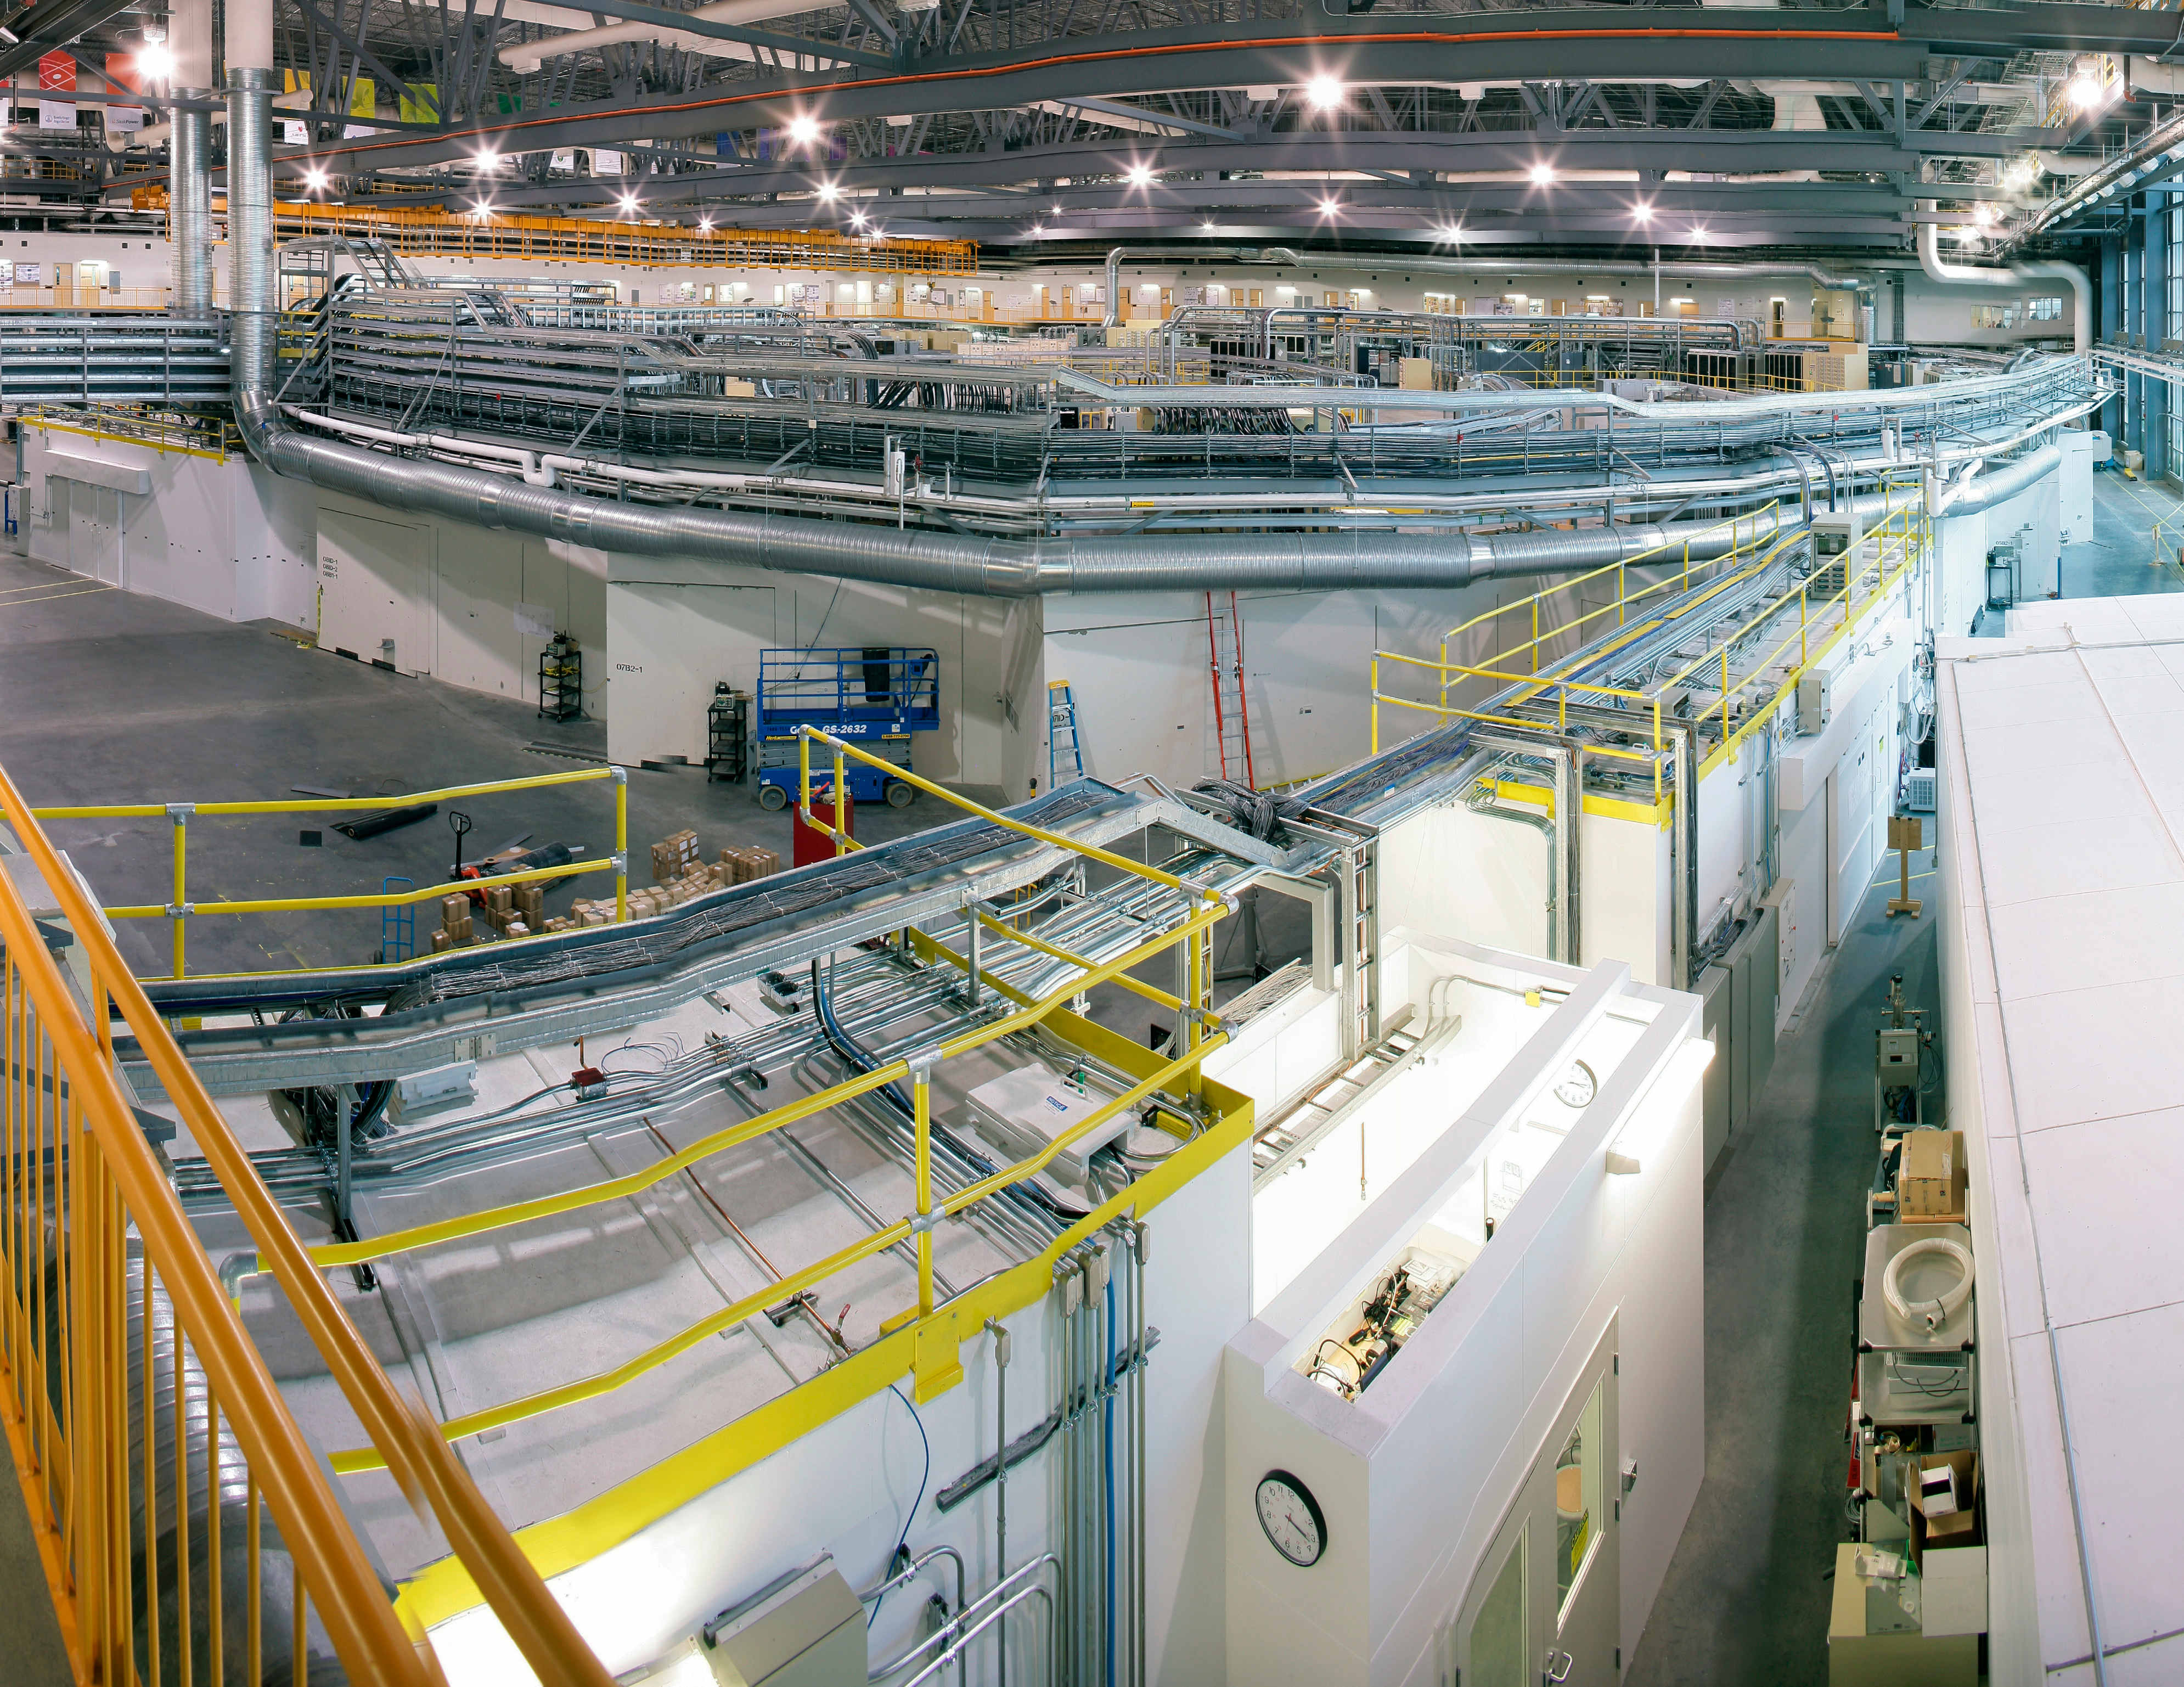
\includegraphics[width=0.8\linewidth]{exp/hxma.jpg}
  \end{center}
\end{frame}

\begin{frame}
  \frametitle{Beamline Optics}

  \begin{description}[Collimating mirror]
  \item[Source] The source can be a bend magnet, a wiggler, or an
    undulator.  XAS beamlines of each sort exist around the world.
  \item[Collimating mirror] Correct the vertical divergence of the
    beam and suppress harmonic content.
  \item[Monochromator] Use Bragg diffraction from a highly perfect
    crystal to select one energy (i.e.\ one wavelength) from the white
    light coming from the source.  Two crystals are needed to direct
    the beam into the hutch.
  \item[Focussing mirror] Change the beam profile from a large
    rectangle to a small circle with minimal reduction of flux.
  \end{description}

  \begin{block}{}
    \begin{center}
      Together these deliver a small, monochromatic, tunable beam into
      the hutch for use in an experiment.
    \end{center}
  \end{block}
\end{frame}

\begin{frame}<1-3| handout:1-3>[label=hutch]
  \frametitle<1| handout:1>{Hutch Instrumentation}
  \frametitle<2| handout:2>{Hutch Instrumentation: Transmission XAS}
  \frametitle<3| handout:3>{Hutch Instrumentation: Fluorescence XAS}
  \frametitle<4| handout:4>{Hutch Instrumentation: Microprobe}

  \begin{center}
\only<1| handout:1>{\includegraphics[width=0.6\linewidth]{exp/hutch_xas.pdf}}%
\only<2| handout:2>{\includegraphics[width=0.6\linewidth]{exp/transmission.pdf}}%
\only<3| handout:3>{\includegraphics[width=0.6\linewidth]{exp/fluorescence.pdf}}%
\only<4| handout:4>{\includegraphics[width=0.6\linewidth]{exp/microprobe.pdf}}
  \end{center}

  \begin{columns}[T]
    \begin{column}{0.5\linewidth}
      \only<1| handout:1>{This is the typical layout of the hutch
        instrumetation.  Depending on the details of the experiment,
        the sample area might include special equipment.}%
      \only<2| handout:2>{In a transmission experiment, we measure the
        direct attenuation of the x-ray beam (Beer's law).
        {\small
          \begin{align}
            I_t =& I_0\exp(-\mu t) \notag\\
            \mu t = & \ln\big(\frac{I_0}{I_t}\big) \notag
          \end{align}
        }%
        Ion chambers are easy to use and accurate over many decades of
        intensity. %
      }%
      \only<3| handout:3>{The fluorescence detector might be an ion
        chamber or it might be an energy discriminating detector. %
        {\small
          \begin{align}
            I_f \propto& \mu I_0 \notag\\
            \mu \propto& \frac{I_f}{I_0} \notag
          \end{align}
        }%
        The energy discriminating detector is useful for low
        concentrations or very heterogeneous samples.
      }
      \only<4| handout:4>{
        \small%
        The energy discriminating detector can see all elements in a
        sample with edges \textit{below} the incident energy.\\
        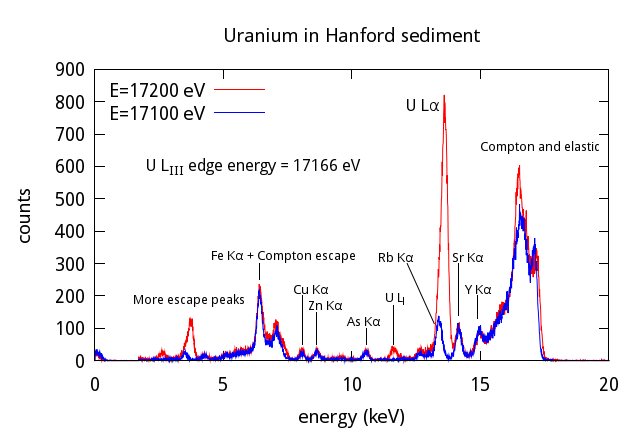
\includegraphics[width=\linewidth]{xrf/xrf.png}
      }%
    \end{column}
    \begin{column}{0.5\linewidth}
      \begin{overlayarea}{\linewidth}{5in}
        \only<1| handout:1>{
          \begin{itemize}
          \item Furnace or cryostat
          \item Electrochemistry or fuel cell
          \item High pressure cell
          \item High field magnet
          \item Peristaltic or stop flow fluid pump
          \item \quad etc...
          \end{itemize}
        }
        \only<2| handout:2>{\includegraphics[width=\linewidth]{exp/ionchamber.pdf}}
        \only<3-4| handout:3-4>{\quad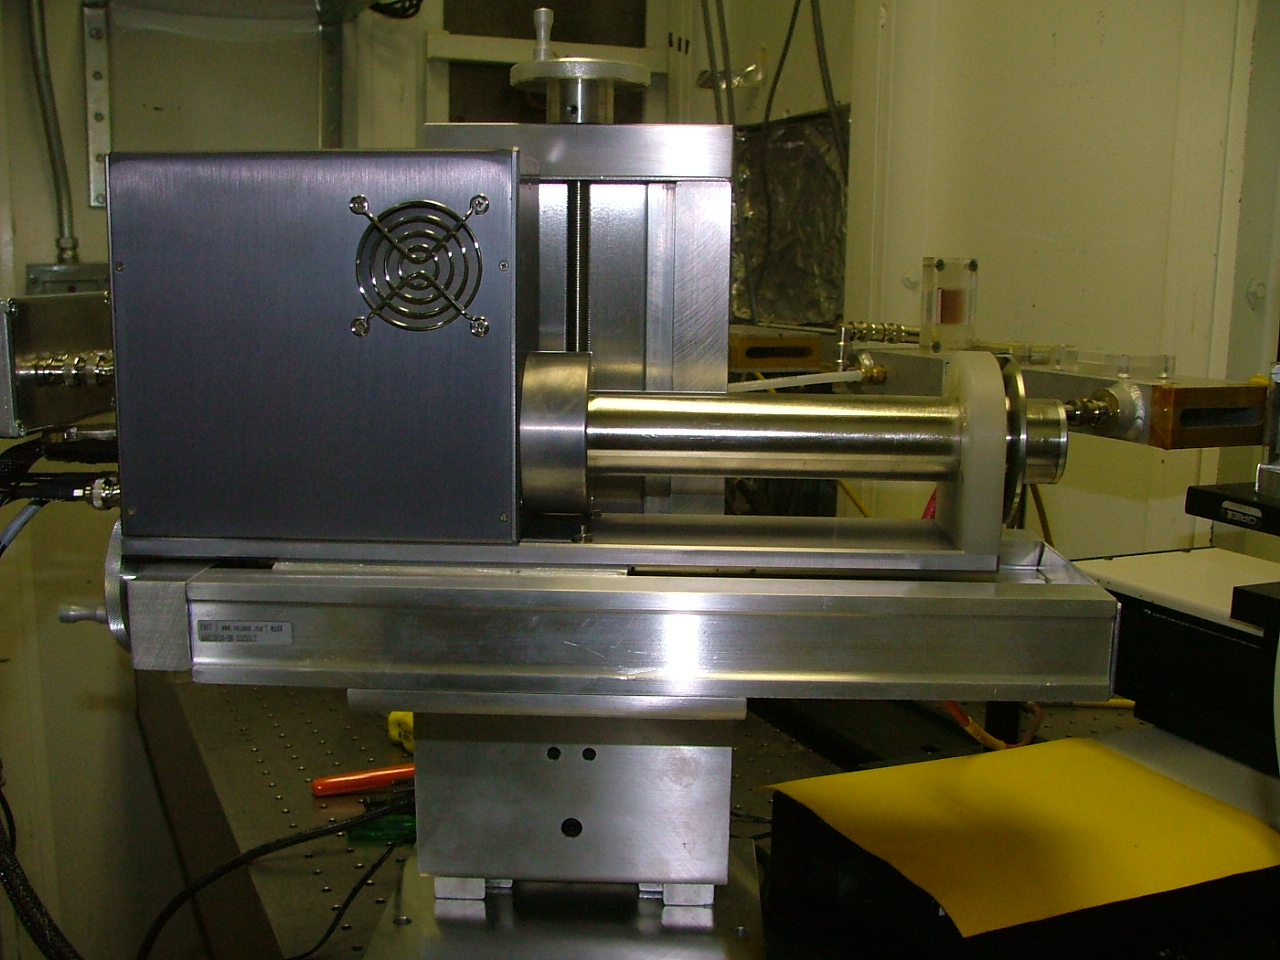
\includegraphics[width=0.8\linewidth]{exp/vortex.png}}
        \only<3| handout:4>{~\\[2ex]This is a \textit{Vortex} 4 element silicon
          drift detector} 
      \end{overlayarea}
    \end{column}
  \end{columns}


\end{frame}


\begin{frame}
  \frametitle{Elements Measured at a Typical Hard X-Ray Beamline}
  \begin{center}
    \includegraphics[width=0.75\linewidth]{images/periodic_table_of_elements.png}

    {\color{SteelBlue3}K-edges, measured with Si(111) monochromator}\\
    {\color{Cyan3}K-edges, measured with Si(311) monochromator}\\
    {\color{Brown4}L-edges}\\[1ex]
    Soft x-ray beamlines exist which deliver photons in the 100\,eV to
    1\,keV range (e.g.\ first row K, transition metal L, actinide N)
  \end{center}
\end{frame}


\section[Real-world problem]{Solving a real-world problem with XRF and XAS}

\begin{frame}
  \frametitle{My backyard}
  When I bought my house, there was a wooden deck off the dining
  room.  I replaced this with a paving stone patio and converted the
  adjacent plot of ground into a vegetable garden.

  \medskip

  \begin{columns}[T]
    \begin{column}{0.5\linewidth}
      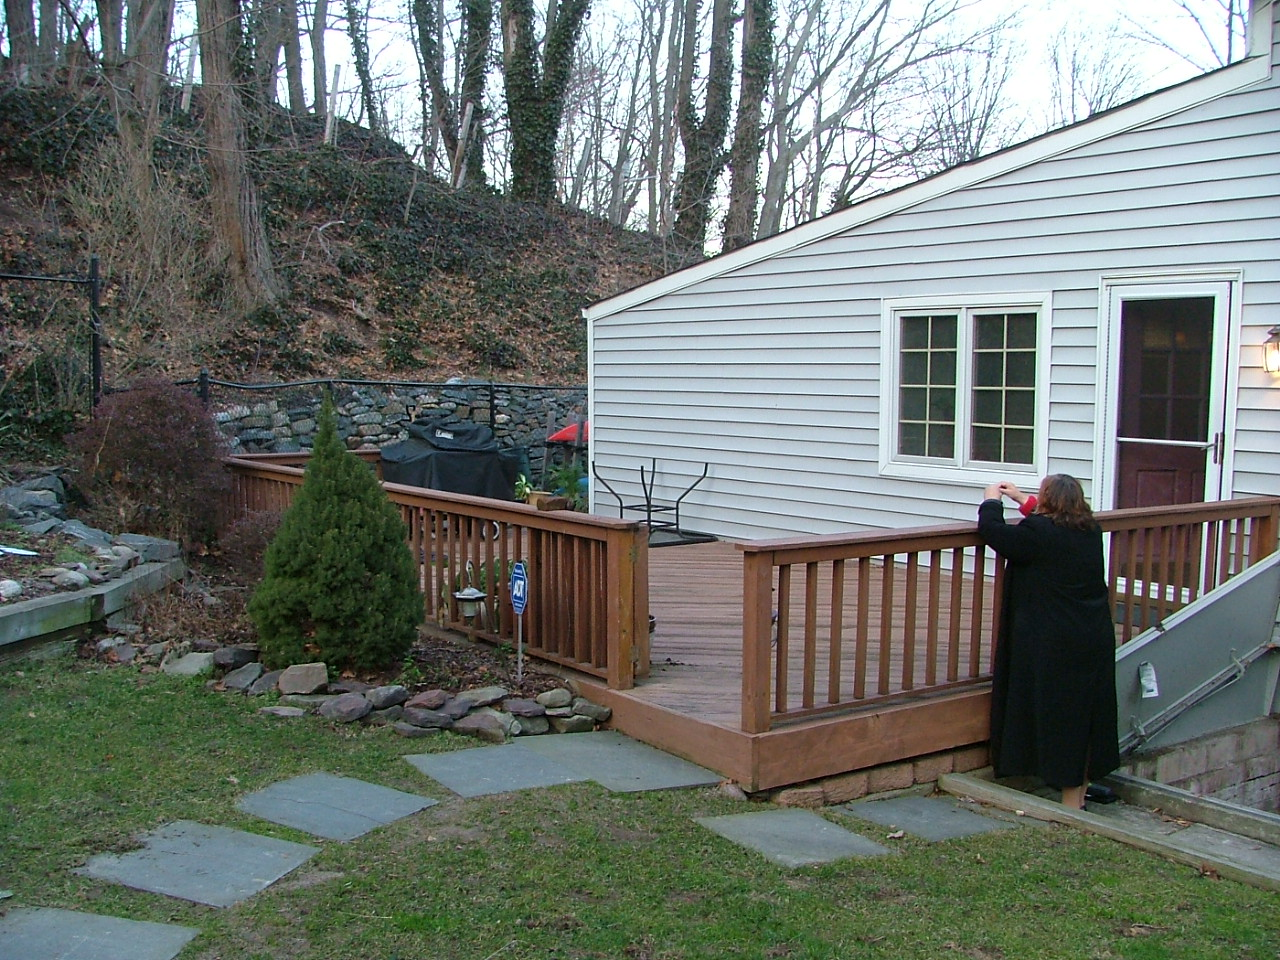
\includegraphics[width=\linewidth]{garden/wooden_deck.jpg}      
    \end{column}
    \begin{column}{0.5\linewidth}
      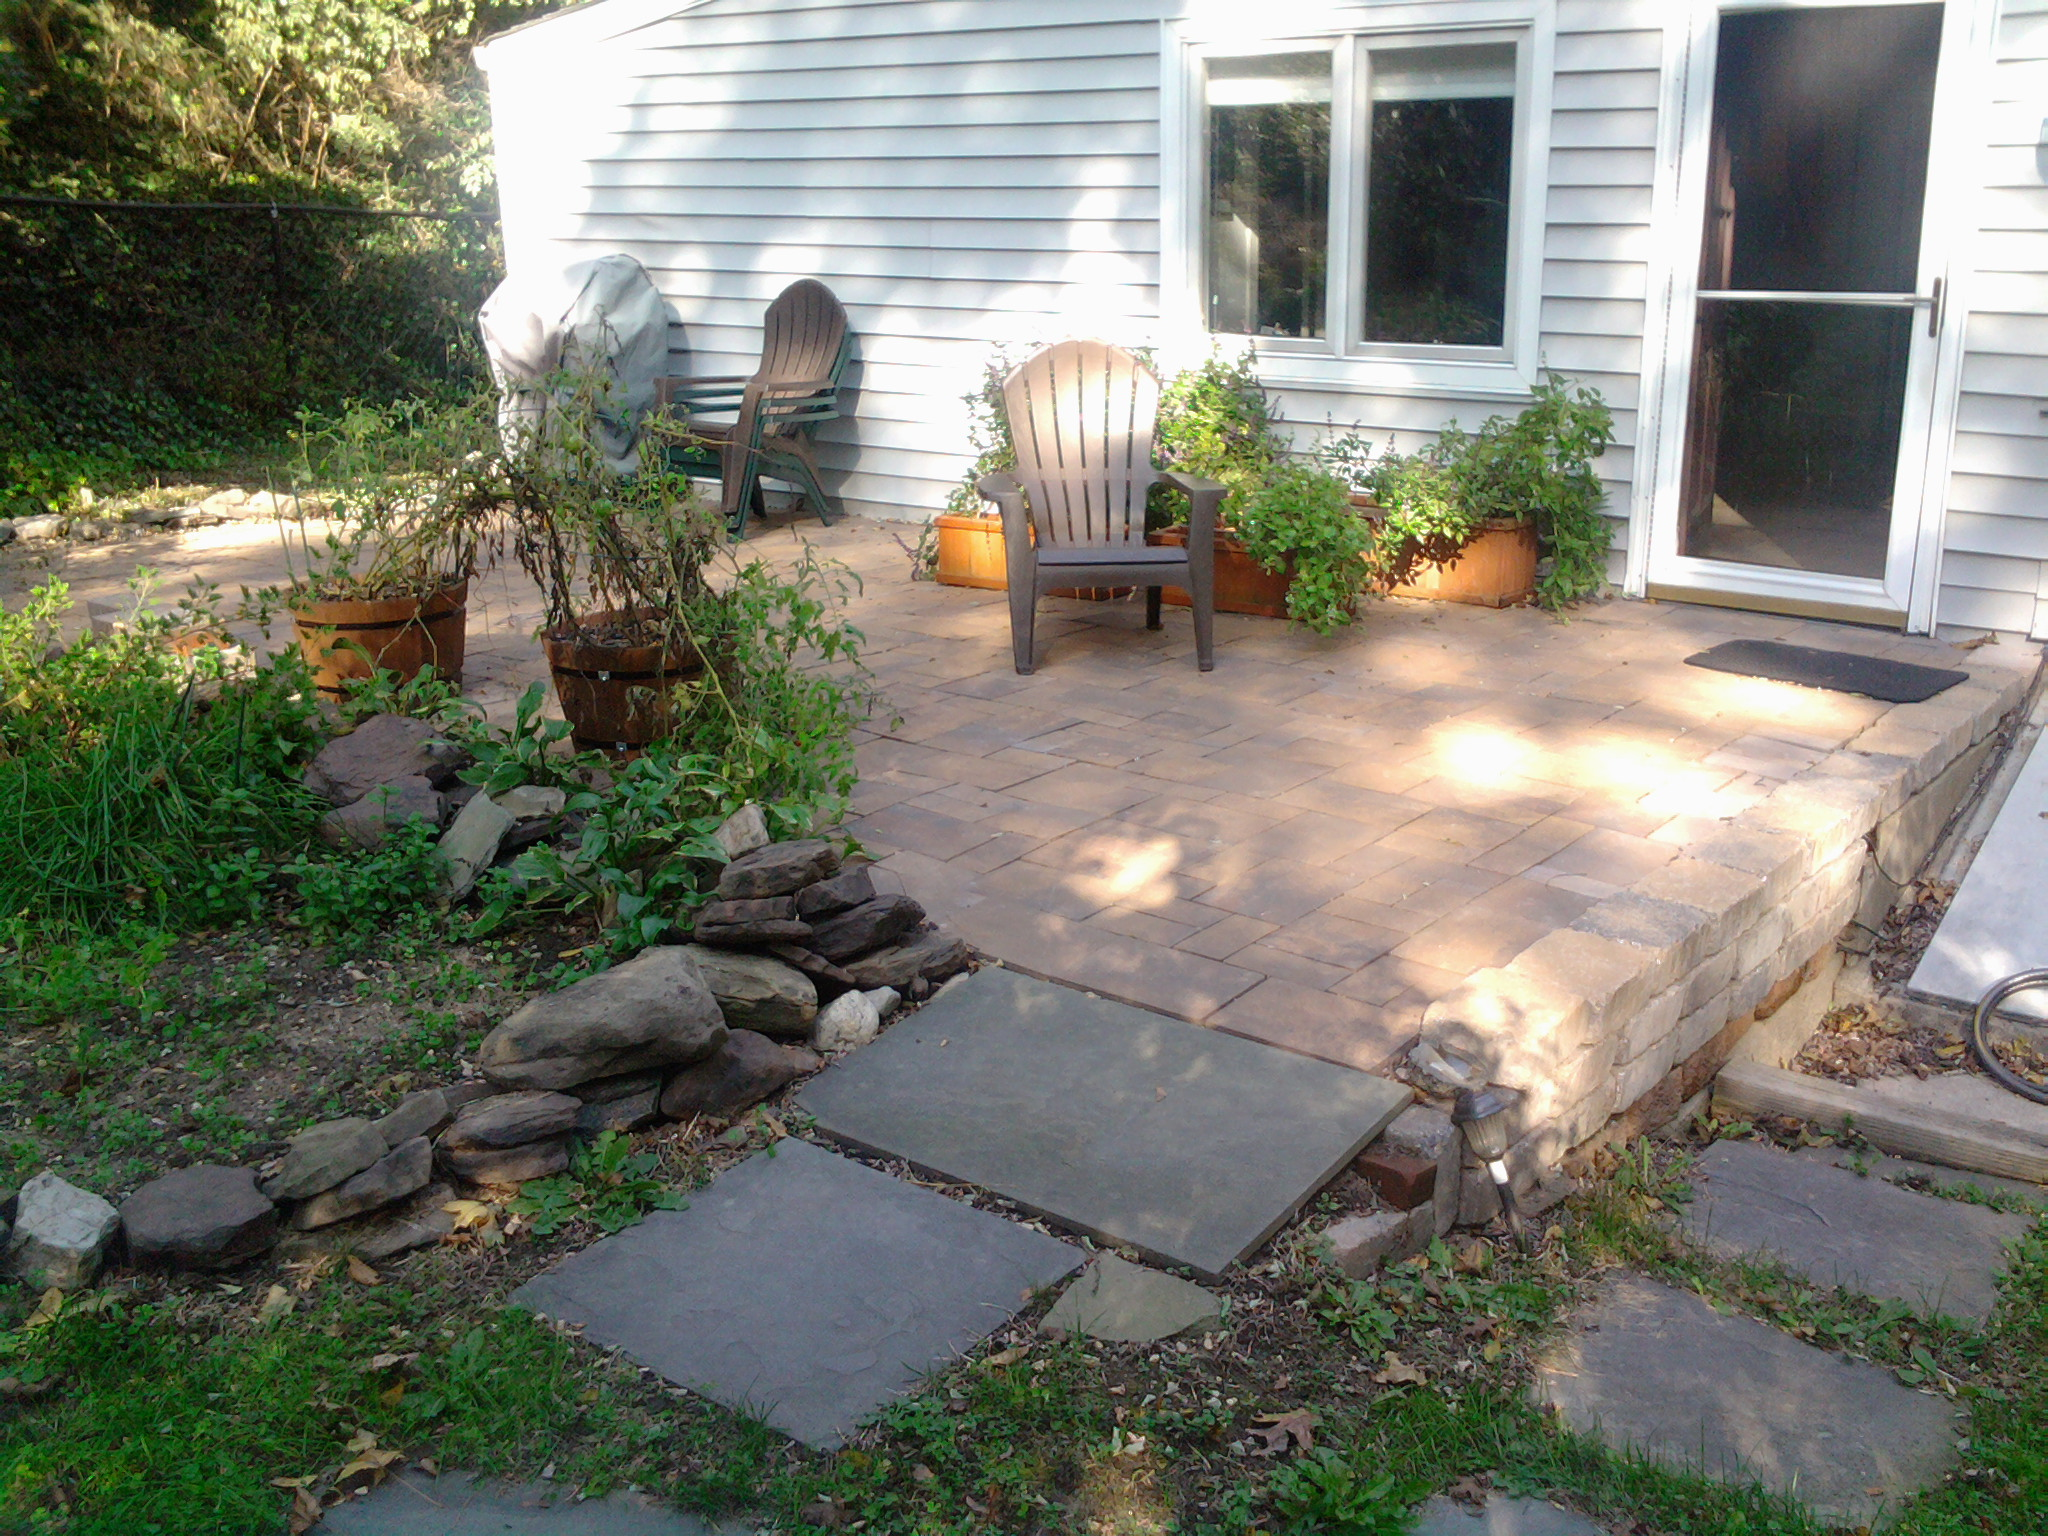
\includegraphics[width=\linewidth]{garden/stone_deck.jpg}
    \end{column}
  \end{columns}
\end{frame}

\begin{frame}
  \frametitle{Wood preservative}

  \begin{columns}[T]
    \begin{column}{0.6\linewidth}
      The wood used to make the deck was treated with the wood
      preservative chromated copper arsentate (CCA), which is chromium
      bearing analogue of copper orthoarsente,
      Cu$_3$(AsO$_4$)$_2$$\cdot$4H$_2$O.
    \end{column}
    \begin{column}{0.4\linewidth}
      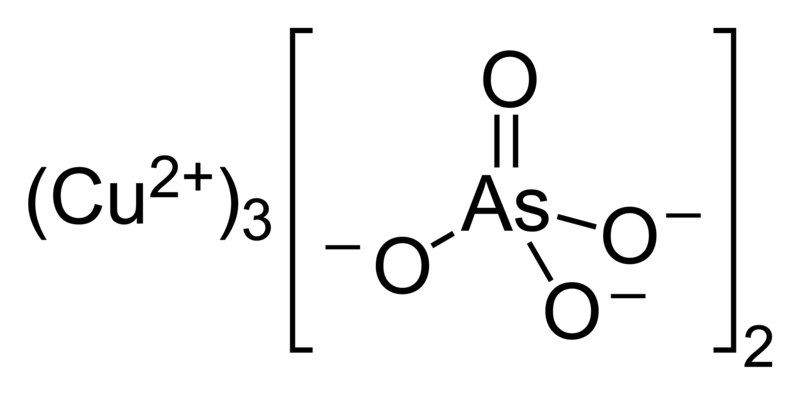
\includegraphics[width=\linewidth]{garden/copper_arsenate.png}      
    \end{column}
  \end{columns}

  \bigskip

  \begin{block}{}
    CCA-treated wood is known to leach all three elements into
    surrounding soils.  I had some questions:

    \bigskip

    \begin{enumerate}
    \item How much As is in the soil?  Is it higher than elsewhere
      in the garden? (Use XRF)
    \item What chemical species is the As in the soil?  (Use XAS)
    \end{enumerate}
  \end{block}
  \begin{textblock*}{0.5\linewidth}(0pt,19.5\TPVertModule)%
    \tiny%
    The orthoarsenate image is from Wikimedia commons and is in the
    public domain.
  \end{textblock*}
\end{frame}

\begin{frame}
  \frametitle{XRF spectra}
  
  I took soil samples from a few centimeters below the surface from a
  spot adjecent to the old deck and from a spot 5 meters away and slightly
  uphill.

  \smallskip

  Here are the XRF spectra from those two spots:

  \begin{center}
    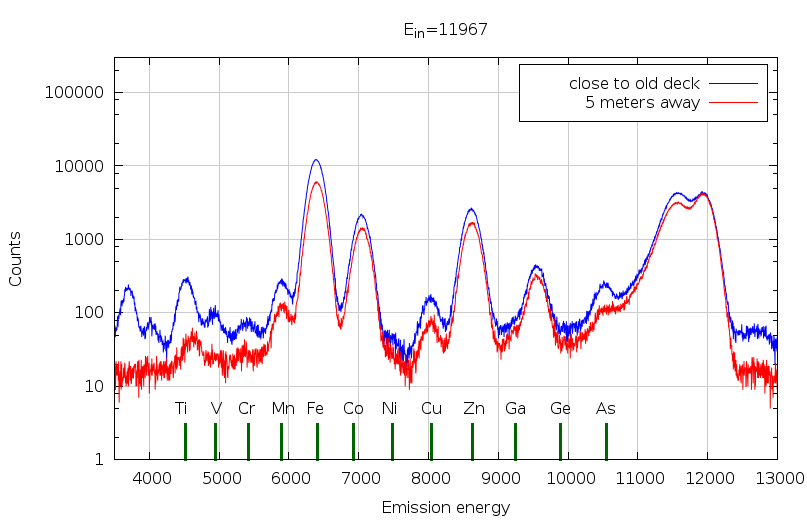
\includegraphics[width=0.65\linewidth]{garden/close_far.png}
  \end{center}

  There is a clear enhancement of both As and Cr in the soil adjacent
  to the old deck.  The As is enhanced roughly two-fold.
\end{frame}

\begin{frame}
  \frametitle{As standards}
  
  As a point of reference, here are the XAS spectra from two inorganic
  As standards, As$^{3+}_2$O$_3$ and As$^{5+}_2$O$_5$.

  \begin{center}
    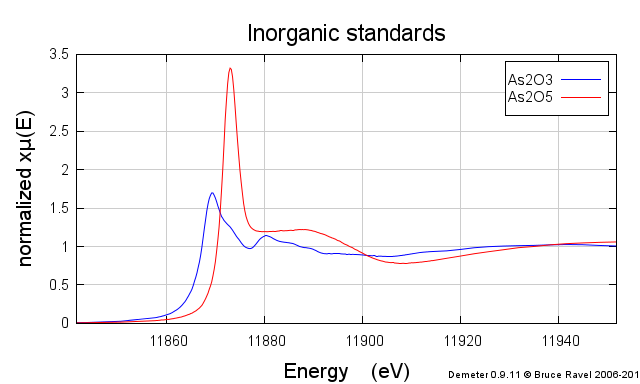
\includegraphics[width=0.65\linewidth]{garden/standards.png}
  \end{center}

  Note that the edge of As$^{5+}$ standard is shifted substantially to
  higher energy and that its white line is much enhanced.

  \begin{center}
    As$^{5+}$ is water soluble, thus more mobile than As$^{3+}$.

    Also As$^{5+}$ is \alert{quite toxic}.
  \end{center}

\end{frame}

\begin{frame}
  \frametitle{XAS from the soil samples}

  \begin{columns}[T]
    \begin{column}{0.5\linewidth}
      Here are the raw $\mu(E)$ data from the two soil locations.
      Sure enough, the signal from the site adjacent to the old deck
      is enhanced by about a factor of 2.
    \end{column}
    \begin{column}{0.5\linewidth}
      \only<2>{ Here are the normalized data compared to standards.
        The As is slightly reduced, but predominantly As$^{5+}$.  As
        in soil is well known to bind to soil particles as As$^{5+}$.}
    \end{column}
  \end{columns}

  \medskip

  \begin{columns}[T]
    \begin{column}{0.5\linewidth}
      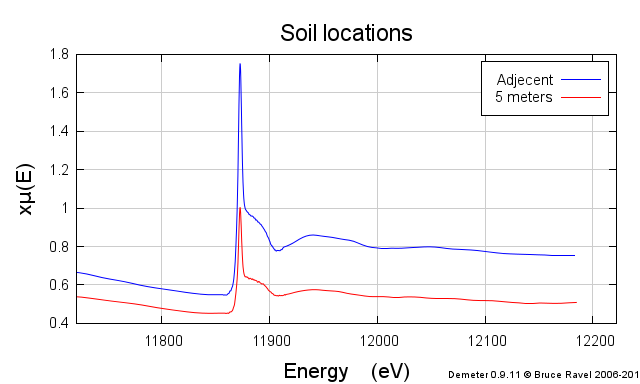
\includegraphics[width=\linewidth]{garden/mue.png}
    \end{column}
    \begin{column}{0.5\linewidth}
      \includegraphics<2>[width=\linewidth]{garden/soils.png}      
    \end{column}
  \end{columns}

  \begin{alertblock}<2>{}
    Should I be worried about the produce I grow in the garden?
  \end{alertblock}
\end{frame}

\begin{frame}
  \frametitle{XRF spectra from plant leaves}
  Here are XRF spectra from the leaf of a squash plant growing in the
  soil adjacent to the old deck.
  \begin{center}
    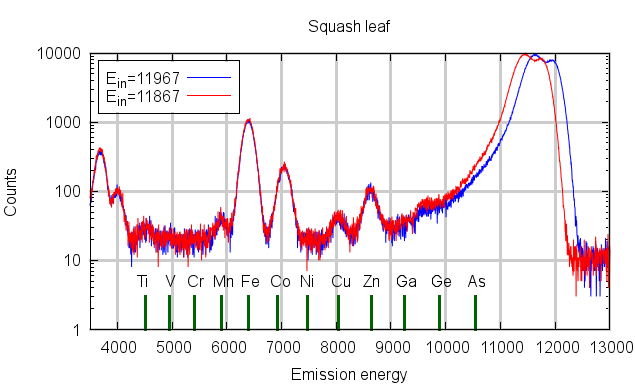
\includegraphics[width=0.65\linewidth]{garden/squash_leaf.png}
  \end{center}
  Although toxic As$^{5+}$ is present in the soil in elevated
  quantities, very little is taken up by the plants growing that
  soil.

  \bigskip

  The squash were delicious!
\end{frame}

\section[XAS Applications]{Applications of XAS}

\begin{frame}
  \frametitle{XAS Examples}

  XAS is used in an amazingly wide variety of disciplines.  Here are
  a few examples from my work in the past few years.

  \bigskip

  \begin{description}[Dielectric materials]
  \item[Economic geology] Measure the rate of reduction of Au$^{3+}$
    chloride to metallic Au and identify an intermediate species
  %\item[Minerology] Supporting evidence for a novel U$^5$/U$^6$
  %  mineral formed under certain hydrothermal conditions
  %\item[Dielectric materials] {\bton} represents a class of materials
  %  with tunable dielectric properties
  \end{description}

  \bigskip

  XAS beamlines regularly see experiments on magnetic materials,
  {\small superconductors}, {\footnotesize materials for recording
    media}, {\scriptsize metallo-organic compounds}, {\tiny
    metalloproteins, {\color{SlateGray4}Earth mantel materials},
    {\color{SlateGray3}extraterrestrial materials},
    {\color{SlateGray2}liquids and amorphous solids},
    {\color{SlateGray1}etc., etc., etc....}}
\end{frame}

\subsection[Economic geology]{Economic geology}
\begin{frame}
  \frametitle{Economic geology (I)}

  One way that gold deposits form is by having Au chloride fluids rise
  from the deep earth, wash over cyanobacteria colonies, and reduce to
  metallic gold.

  \begin{columns}
    \begin{column}{0.5\linewidth}
      \includegraphics[width=\linewidth]{aucl/aucl_exp.pdf}
    \end{column}
    \begin{column}{0.5\linewidth}
      We simulated this process at the beamline by exposing
      cyanobacteria to an Au$^{3+}$ solution and ``watching'' the
      evolution of the Au XAS from Au$^{3+}$ to Au$^0$.
      \begin{block}{Questions}
        \begin{itemize}
        \item What is the rate constant?
        \item Is there an intermediate species?
        \end{itemize}
      \end{block}
    \end{column}
  \end{columns}

  \begin{textblock*}{0.5\linewidth}(0pt,18.5\TPVertModule) 
    \tiny
    M. Lengke et el., \textit{Mechanisms of Gold Bioaccumulation by
      Filamentous Cyanobacteria from Gold(III)-Chloride Complex},
    Environ. Sci. Technol. \textbf{40}(20) p.~6304-6309. (2006),
    \href{http://dx.doi.org/10.1021/es061040r}
    {\color{Blue4}\texttt{DOI: 10.1021/es061040r}}
  \end{textblock*}
\end{frame}
\begin{frame}
  \frametitle{Economic geology (II)}

  \begin{columns}
    \begin{column}{0.5\linewidth}
      We see that \alert{7 minutes} after injection, the data strongly
      resemble the {\color{Blue3}Au$^{3+}$Cl}.  After
      {\color{Purple4}one week}, the data resemble
      {\color{Green4}Au metal}.\\[1ex]
      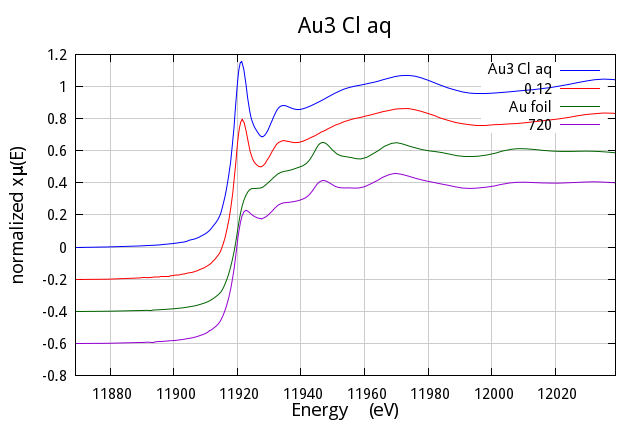
\includegraphics[width=\linewidth]{aucl/aucl_data.png}
    \end{column}
    \begin{column}{0.5\linewidth}
      Over the course of the time series, the white line $\sim11921$
      shrinks while the bump $\sim11945$ grows, suggesting the
      reduction to Au metal.\\[1ex]
      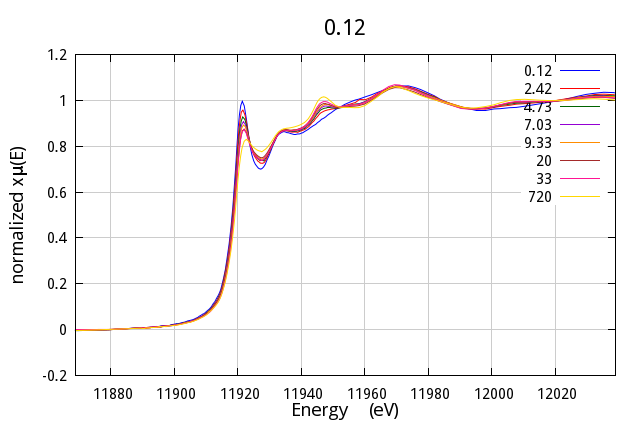
\includegraphics[width=\linewidth]{aucl/aucl_time.png}
    \end{column}
  \end{columns}

  \begin{textblock*}{0.5\linewidth}(0pt,18.5\TPVertModule) 
    \tiny
    M. Lengke et el., \textit{Mechanisms of Gold Bioaccumulation by
      Filamentous Cyanobacteria from Gold(III)-Chloride Complex},
    Environ. Sci. Technol. \textbf{40}(20) p.~6304-6309. (2006),
    \href{http://dx.doi.org/10.1021/es061040r}
    {\color{Blue4}\texttt{DOI: 10.1021/es061040r}}
  \end{textblock*}
\end{frame}
\begin{frame}
  \frametitle{Economic geology (III)}

  \begin{columns}
    \begin{column}{0.5\linewidth}
      We can analyze these data as a linear combination of species,
      including {\color{Green4}Au$^{3+}$Cl}, {\color{Purple4}Au
        metal}, and {\color{Orange2}Au$^{1+}$ sulfide}.\\[1ex]
      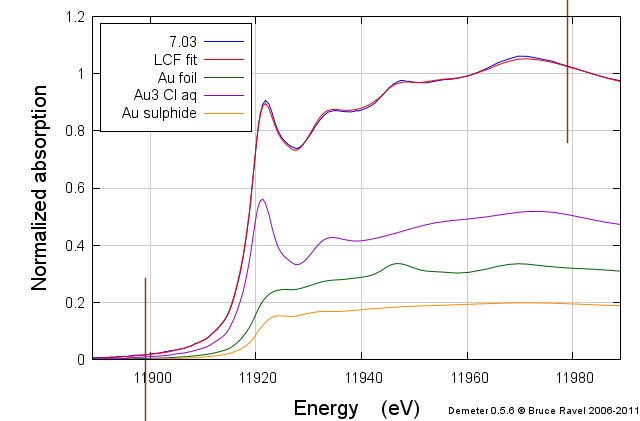
\includegraphics[width=\linewidth]{aucl/aucl_lcf.png}
    \end{column}
    \begin{column}{0.5\linewidth}
      We can plot out the contributions from these species as a
      function of time to get a sense of reaction rates.\\[1ex]
      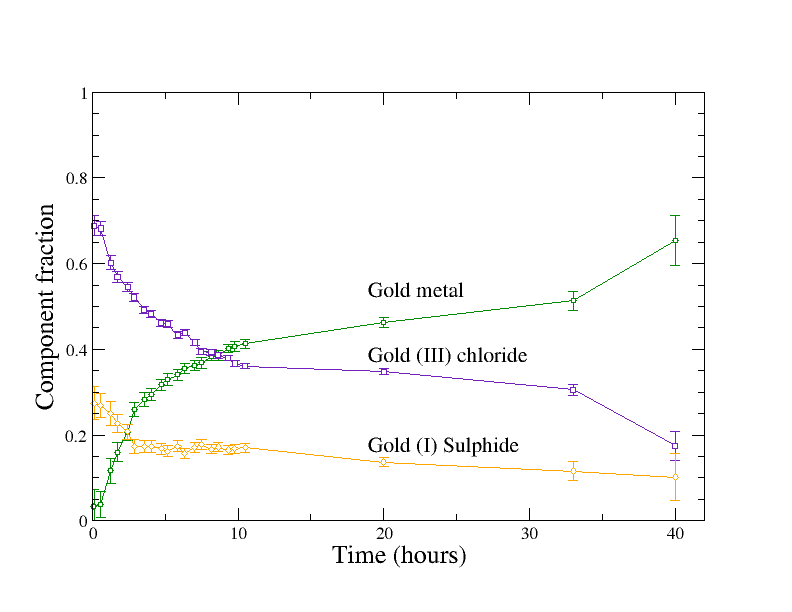
\includegraphics[width=\linewidth]{aucl/aucl_results.png}
    \end{column}
  \end{columns}

  \begin{textblock*}{0.5\linewidth}(0pt,18.5\TPVertModule) 
    \tiny
    M. Lengke et el., \textit{Mechanisms of Gold Bioaccumulation by
      Filamentous Cyanobacteria from Gold(III)-Chloride Complex},
    Environ. Sci. Technol. \textbf{40}(20) p.~6304-6309. (2006),
    \href{http://dx.doi.org/10.1021/es061040r}
    {\color{Blue4}\texttt{DOI: 10.1021/es061040r}}
  \end{textblock*}
\end{frame}


%\subsection[Minerology]{Minerology}
\begin{frame}
  \frametitle{Minerology (I)}

  A deep understanding of the nuclear fuel cycle requires study of
  ``exotic'' pentavalent uranium minerals that can form under specific
  mine or storage facility conditions.  One such mineral,
  {\ufivemineral}, has recently been synthesized.

  \qquad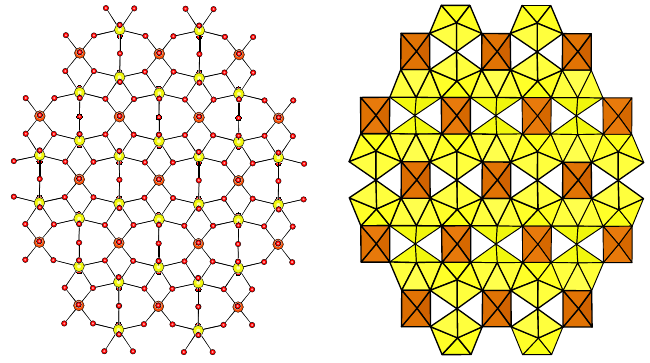
\includegraphics[width=0.7\linewidth]{xas/u5mineral.png}

  \begin{block}{}
    XRD is an indirect measure of valence | XAS is a direct measure!
  \end{block}

  \begin{bottomnote}[0.5][19]
    N. Belai et el., \textit{Pentavalent Uranium Oxide via Reduction
    of [UO$_2$]$^{2+}$ Under Hydrothermal Reaction Conditions},
    Inorg. Chem., 2008, 47 (21), pp 10135--10140,
    \doiref{10.1021/ic801534m}[LightBlue4]
  \end{bottomnote}
\end{frame}
\begin{frame}
  \frametitle{Minerology (II)}
  XAS on \ufivemineral

  \begin{columns}[T]
    \begin{column}{0.5\linewidth}
      \begin{center}
        \small
        XANES data\\
        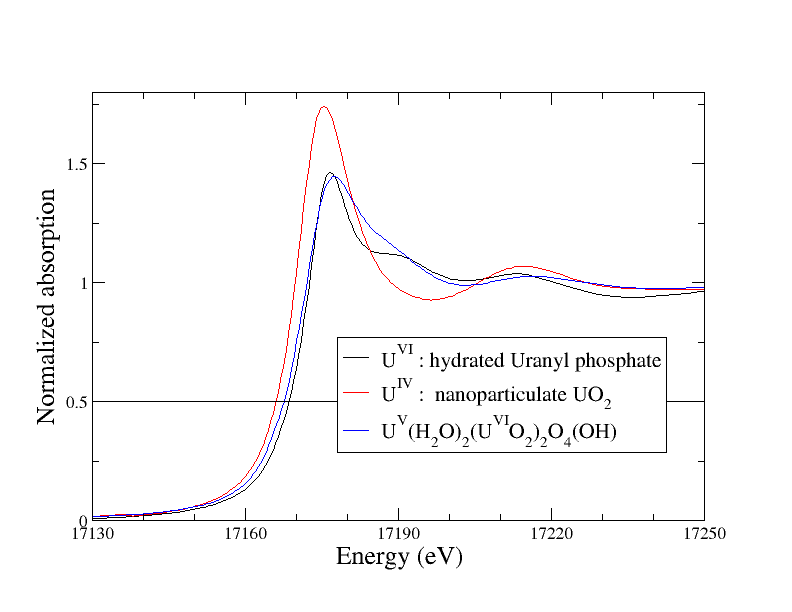
\includegraphics[width=\linewidth]{xas/u5norm.png}\\
        We see evidence of U$^{\mathrm{V}}$ by  the intermediate edge position
        between our U$^{\mathrm{IV}}$ and U$^{\mathrm{VI}}$ standards.
      \end{center}
    \end{column}
    \begin{column}{0.5\linewidth}
      \begin{center}
        \small
        EXAFS analysis\\
        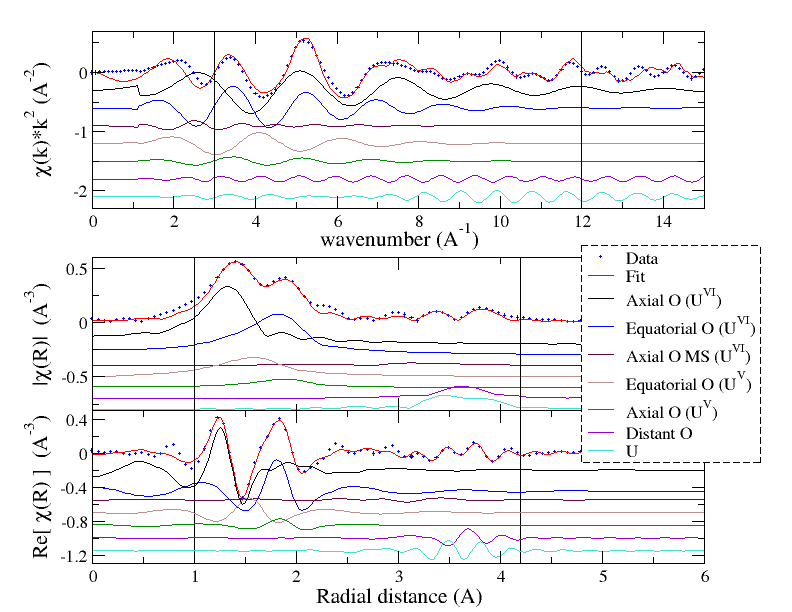
\includegraphics[width=\linewidth]{xas/u5chikr.png}\\
        The crystal structure refined from the XRD is consistent with
        the EXAFS data.
      \end{center}
    \end{column}
  \end{columns}

%   \bigskip

%   The data on this page has been redacted as the paper has not yet
%   been published.  The data that were here demonstrated that the
%   mineral contains U$^{\mathrm{V}}$ and that the structure refined
%   from XRD is consistent with the EXAFS data.

  \begin{bottomnote}[0.5][19]
    N. Belai et el., \textit{Pentavalent Uranium Oxide via Reduction
    of [UO$_2$]$^{2+}$ Under Hydrothermal Reaction Conditions},
    Inorg. Chem., 2008, 47 (21), pp 10135--10140,
    \doiref{10.1021/ic801534m}[LightBlue4]
  \end{bottomnote}
\end{frame}



%
\subsection[Dielectric materials]{Dielectric materials}
\begin{frame}
  \frametitle{Dielectric materials (I)}

  Tantalum oxynitrides are a class of dielectric materials with high
  $K$ which is tunable by selection of the A cation.  By mixing A
  cations, a temperature-constant dielectric is possible.
  \begin{columns}
    \begin{column}{0.5\linewidth}
      \begin{center}
        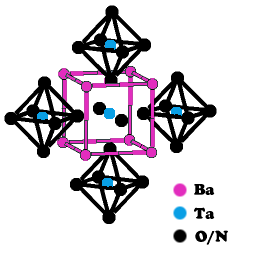
\includegraphics[width=0.6\linewidth]{xas/perovskite.png}
      \end{center}
    \end{column}
    \begin{column}{0.5\linewidth}
      \begin{center}
        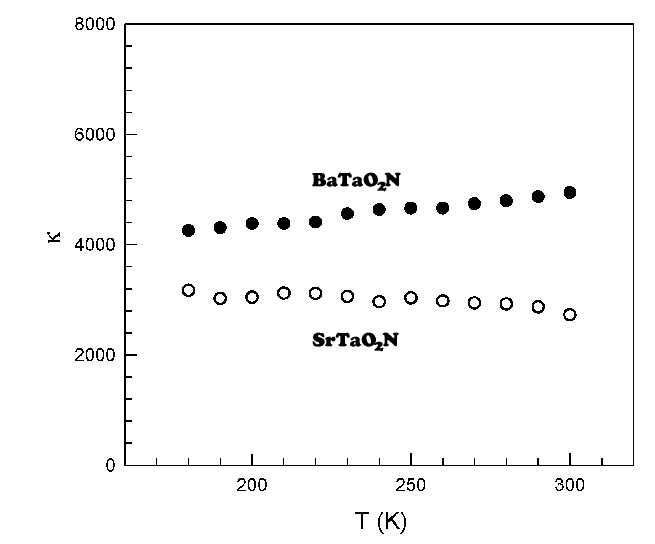
\includegraphics[width=0.9\linewidth]{xas/bton_permit.png}
      \end{center}
    \end{column}
  \end{columns}

  First principles DFT suggests that the different ionic radii of O
  and N introduce substantial disorder around the Ta atom.
  
  \begin{textblock*}{0.5\linewidth}(0pt,19\TPVertModule) 
    \tiny
    B. Ravel et el., \textit{Role of local disorder in the dielectric
      response of BaTaO$_2$N}, Phys. Rev. \textbf{B73}, p. 184121 (2006),
    \href{http://dx.doi.org/10.1103/PhysRevB.73.184121}
    {\color{Blue4}\texttt{DOI: 10.1103/PhysRevB.73.184121}}
  \end{textblock*}
\end{frame}

\begin{frame}
  \frametitle{Dielectric materials (II)}%
  The DFT results in a rather complex coordination environment about
  the Ta atom | much more complex than the simple perovskite
  structure.
  \begin{columns}
    \begin{column}{0.5\linewidth}
      \begin{center}
        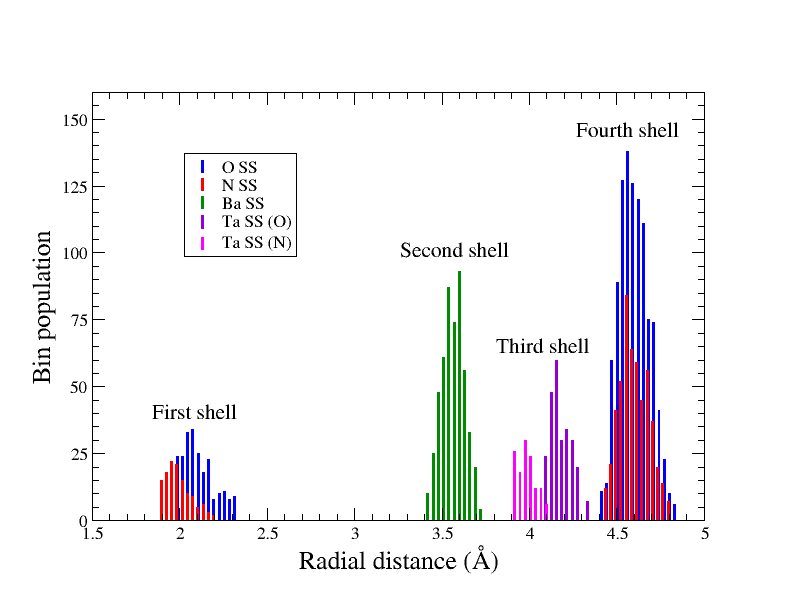
\includegraphics[width=\linewidth]{xas/bton_SS.png}
      \end{center}
    \end{column}
    \begin{column}{0.5\linewidth}
      \begin{center}
        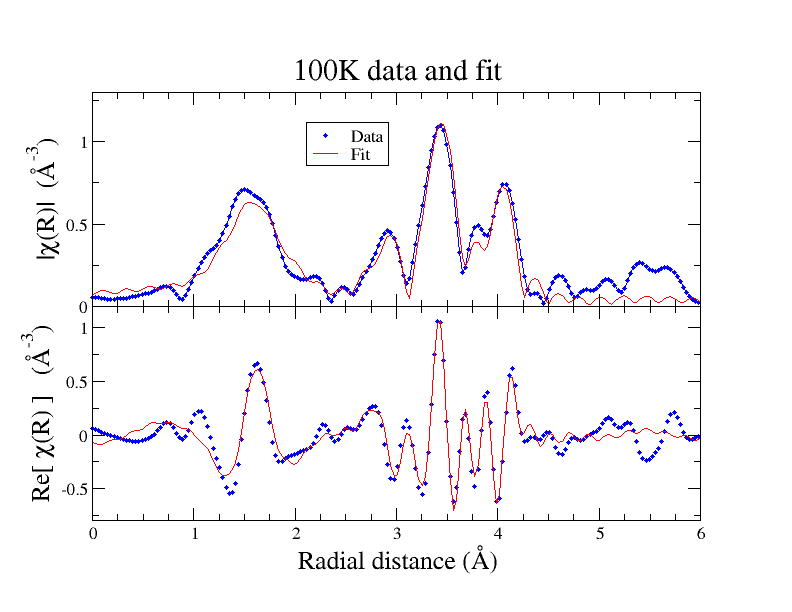
\includegraphics[width=\linewidth]{xas/bton_fit.png}
      \end{center}
    \end{column}
  \end{columns}
  With some effort, this complexity can be incorporated into the data
  analysis.  The EXAFS data are shown to be (mostly) consistent with
  the DFT results.

  \begin{textblock*}{0.5\linewidth}(0pt,19\TPVertModule) 
    \tiny
    B. Ravel et al., \textit{Role of local disorder in the dielectric
      response of BaTaO$_2$N}, Phys. Rev. \textbf{B73}, p. 184121 (2006), 
    \href{http://dx.doi.org/10.1103/PhysRevB.73.184121}
    {\color{Blue4}\texttt{DOI: 10.1103/PhysRevB.73.184121}}
  \end{textblock*}
\end{frame}



\section[Microprobe]{XRF and XAS on the Micron Scale}

\againframe<4| handout:4>{hutch}

\begin{frame}
  \frametitle{Focussing optics}

  Different types of focussing optics can be matched to the relevant
  length scales of different samples

  \begin{columns}
    \begin{column}{0.6\linewidth}
      \begin{description}[Refrac]
      \item[1D focussing + slits] A total external reflection mirror
        is bent to condense the x-rays vertically.  Slits are used to
        define the horizontal extent. ($>50\,\mu$m)
      \item[Kirkpatrick-Baez mirrors] Short mirrors with excellent
        figures are used in both directions to define a small
        spot. (1--25 $\mu$m)
      \item[Refractive optics] Fresnel zone plates use refraction to
        define a small first order spot ($<1\,\mu$m)
      \end{description}
    \end{column}
    \begin{column}{0.4\linewidth}
      \begin{center}
        \includegraphics[width=0.9\linewidth]{xrf/kb.png}\\[1ex]
        \includegraphics[width=0.7\linewidth]{xrf/zp.png}
      \end{center}

    \end{column}
  \end{columns}
\end{frame}

\begin{frame}
  \frametitle{X-ray Fluorescence Mapping}

  \begin{columns}
    \begin{column}{0.5\linewidth}
      \includegraphics[width=0.9\linewidth]{xrf/raster.jpg}
    \end{column}
    \begin{column}{0.5\linewidth}
      The mapping experiment involves placing the sample on an
      3-dimensional stage and in the focal spot of the beam.

      \bigskip

      The sample is rastered in $\hat{y}$ and $\hat{z}$ to cover a
      two-dimensional area.

      \bigskip

      At each point $\overline{xy}$, the XRF spectrum is measured.
      Integrating the elemetal regions of interest yields maps of the
      elemental distributions.
    \end{column}
  \end{columns}
\end{frame}

\subsection[200 $\mu$m]{200 Micron Probe}

\begin{frame}
  \frametitle{Gravel Contaminated with U}

  \begin{center}
    Gravel embedded in epoxy with a polished surface\\[1ex]

    \only<1| handout:1>{Under a UV lamp, U glows greenish.}
    \only<2| handout:2>{UV photo + superposed U map | 200\,$\mu$m probe at APS 10ID.}
    \\[1ex]

    \only<1| handout:1>{\includegraphics[width=0.75\linewidth]{xrf/pebble.png}}
    \only<2| handout:2>{\includegraphics[width=0.75\linewidth]{xrf/pebblespot.png}}
  \end{center}

  \begin{textblock*}{0.5\linewidth}(0pt,19.75\TPVertModule) \tiny
    D. Phillips et el., Env. Sci. and Tech., 2008, 42 (19), pp
    7104–7110
    \href{http://dx.doi.org/10.1021/es8001579}{\color{Blue4}\texttt{DOI:
        10.1021/es8001579}}
  \end{textblock*}
\end{frame}
\begin{frame}
  \frametitle{XRF Spectra at each Position}

  Here are a few of the XRF spectra from the marked area on the U map
  from the previous page.
  \begin{center}
    \includegraphics[width=0.7\linewidth]{xrf/beanx=4000.png}
  \end{center}
  \begin{textblock*}{0.5\linewidth}(0pt,19.75\TPVertModule) \tiny
    D. Phillips et el., Env. Sci. and Tech., 2008, 42 (19), pp
    7104–7110
    \href{http://dx.doi.org/10.1021/es8001579}{\color{Blue4}\texttt{DOI:
        10.1021/es8001579}}
  \end{textblock*}
\end{frame}

\begin{frame}
  \frametitle{$\mu$-EXAFS}

  \begin{columns}[T]
    \begin{column}{0.34\linewidth}
      \visible<1->{\includegraphics[width=\linewidth]{xrf/bean_e}}

      \visible<2->{\includegraphics[width=\linewidth]{xrf/bean_n}}

      \visible<3>{\includegraphics[width=\linewidth]{xrf/bean_r}}
    \end{column}
    \begin{column}{0.66\linewidth}
      \begin{itemize}[<+->]
      \item High quality XAS data is measured with the 200\,$\mu$m
        probe.  We can see the variation in U quantity under the spot
        in the XAS step size.\\[10ex]
      \item Normalizing the data, we see variability in the XANES,
        indicating spatial heterogeneity in U speciation.\\[10ex]
      \item The EXAFS is of high quality and can be analyzed to
        uncover the different structural environments around the U at
        the various locations.
      \end{itemize}
    \end{column}
  \end{columns}
  \begin{textblock*}{0.5\linewidth}(0pt,19.75\TPVertModule) \tiny
    D. Phillips et el., Env. Sci. and Tech., 2008, 42 (19), pp
    7104–7110
    \href{http://dx.doi.org/10.1021/es8001579}{\color{Blue4}\texttt{DOI:
        10.1021/es8001579}}
  \end{textblock*}
\end{frame}

\subsection[20 $\mu$m]{20 Micron Probe}

\begin{frame}
  \frametitle{Arsenic Hyper-Accumulating Plant (I)}

  \begin{center}
    An \textit{Arabadopsis} mutant was plucked from arsenite
    contaminated medium and pressed between two pieces of kapton
    tape.\\[1ex]
    \includegraphics[width=0.8\linewidth]{xrf/delta6200_3.jpg}
  \end{center}
  \begin{textblock*}{0.5\linewidth}(0pt,20\TPVertModule)
    \tiny M. Pischke and B. Ravel, unpublished
  \end{textblock*}
\end{frame}
\begin{frame}
  \frametitle{Arsenic Hyper-Accumulating Plant (II)}

  \begin{columns}[T]
    \begin{column}{0.6\linewidth}
      \qquad\includegraphics[width=0.65\linewidth]{xrf/arabadopsis_sm.png}

      \quad\includegraphics[width=0.7\linewidth]{xrf/arabadopsis_xanes.png}

      \small We measured XANES from a vein in the leaf with a
      20\,$\mu$m probe at APS 13BM.\\
      {\color{Green4}$\sim$25\% As trisglutathiol} and
      {\color{Purple4}$\sim$75\% Arsenite}

    \end{column}
    \begin{column}{0.4\linewidth}
      \includegraphics[width=\linewidth]{xrf/arabadopsis_as.png}

      \includegraphics[width=\linewidth]{xrf/arabadopsis_fe.png}

      \includegraphics[width=\linewidth]{xrf/arabadopsis_zn.png}
    \end{column}
  \end{columns}
  \begin{textblock*}{0.5\linewidth}(0pt,20\TPVertModule)
    \tiny M. Pischke and B. Ravel, unpublished
  \end{textblock*}
\end{frame}

%
\subsection[200 nm]{200 Nanometer Probe}
\begin{frame}
  \frametitle{Radiation resistance of D. Radiodurans (I)}

  \textit{D. Radiodurens} were cultured on a TEM grid and dried.  The
  locations of cells were registered under a light microscope and
  found again at APS beamline 2\,ID-D, where a 250\,nm
  probe was used.
  
  \begin{columns}
    \begin{column}{0.4\linewidth}
      \begin{center}
        \includegraphics[width=0.8\linewidth]{xrf/dr_tem_grid.jpg}\\[1ex]
        {\tiny
          \begin{tabular}{ccc}
            element & max $\mu$g/cm$^2$ & max mass ppm \\
            \hline
            P  & 3.5200 & 312.3\\
            S  & 0.4790 & 42.5\\
            Cl & 0.2130 & 18.9\\
            K  & 2.3600 & 209.4\\
            Ca & 0.1300 & 11.5\\
            Cr & 0.0014 & 0.1\\
            Mn & 0.0155 & 1.4\\
            Fe & 0.0135 & 1.2\\
            Co & 0.0019 & 0.2\\
            Ni & 0.0024 & 0.2\\
            Cu & 0.0413 & 3.7\\
            Zn & 0.0457 & 4.1\\
          \end{tabular}
        }
      \end{center}
    \end{column}
    \begin{column}{0.6\linewidth}
      \begin{center}
        This proved to be a colony of four cells:\\[1ex]
        \includegraphics[width=0.9\linewidth]{xrf/dr_allmaps.png}
      \end{center}
    \end{column}
  \end{columns}

  \bigskip

  \begin{textblock*}{0.5\linewidth}(0pt,19\TPVertModule)
    \tiny M. Daly et el., \textit{Protein Oxidation Implicated as the
      Primary Determinant of Bacterial Radioresistance}, PLoS
    Biol \textbf{5}(4): e92 
    \href{http://dx.doi.org/10.1371/journal.pbio.0050092}
    {\color{Blue4}\texttt{doi:10.1371/journal.pbio.0050092}}
  \end{textblock*}
\end{frame}


\begin{frame}
  \frametitle{Radiation resistance of D. Radiodurans (II)}

  \textit{D. Radiodurens}:
  \begin{enumerate}
  \item is unusually resistent to high doses of ionizing radiation, even
    thriving under doses that would quickly kill other bacteria
  \item has high intracellular Mn/Fe concentration ratios compared to
    IR-sensitive bacteria
  \end{enumerate}

  \bigskip
  
  \begin{block}{We noticed a trend in the Fe and Mn distribution}
    \begin{itemize}
    \item Fe is enhanced in the cell walls.  It is available when
      needed for metabolism but sequestered from cell organs to
      protect them from Fenton chemistry.
    \item Mn in enhanced in cell body and is available to scavange
      radiolosis radicals near cell organs.
    \end{itemize}
  \end{block}

  \bigskip

  \begin{textblock*}{0.5\linewidth}(0pt,19\TPVertModule)
    \tiny M. Daly et el., \textit{Protein Oxidation Implicated as the
      Primary Determinant of Bacterial Radioresistance}, PLoS
    Biol \textbf{5}(4): e92
    \href{http://dx.doi.org/10.1371/journal.pbio.0050092}
    {\color{Blue4}\texttt{doi:10.1371/journal.pbio.0050092}}
  \end{textblock*}
\end{frame}

\begin{frame}
  \frametitle{Radiation resistance of D. Radiodurans (III)}

  Here are images we published on a diploid colony:

  \bigskip

  \begin{columns}
    \begin{column}{0.5\linewidth}
      \includegraphics[width=\linewidth]{xrf/dr_4maps.jpg}
    \end{column}
    \begin{column}{0.5\linewidth}
      Superposing those four images:\\[1ex]
      \includegraphics[width=\linewidth]{xrf/dr_superposed.jpg}
    \end{column}
  \end{columns}    
  
  \bigskip

  \begin{textblock*}{0.5\linewidth}(0pt,19\TPVertModule)
    \tiny M. Daly et el., \textit{Protein Oxidation Implicated as the
      Primary Determinant of Bacterial Radioresistance}, PLoS
    Biol \textbf{5}(4): e92
    \href{http://dx.doi.org/10.1371/journal.pbio.0050092}
    {\color{Blue4}\texttt{doi:10.1371/journal.pbio.0050092}}
  \end{textblock*}
\end{frame}

    % deinococus radiodurans example

\section[XAS Community]{The XAS Community}

\begin{frame}
  \frametitle{Where to go for more information}
  \begin{center}
    {\LARGE \texttt{http://xafs.org/}}\\[1ex]
    \includegraphics[width=0.95\linewidth]{images/xafsorg.png}
  \end{center}
\end{frame}

\begin{frame}
  \frametitle{Information about the software}
  \begin{description}[Ifeffit]
  \item[Ifeffit] A suite of interactive programs for XAFS analysis,
    combining high-quality and well-tested XAFS analysis algorithms,
    tools for general data manipulation, and graphical display of
    data.\\\qquad{\scriptsize
      \href{http://cars9.uchicago.edu/ifeffit/}
      {\color{Blue4}\texttt{http://cars9.uchicago.edu/ifeffit/}}}
  \item[Athena \& Artemis] Graphical programs for the processing and
    analysis of XAFS data.\\\qquad{\scriptsize
      \href{http://bruceravel.github.com/demeter}
      {\color{Blue4}\texttt{http://bruceravel.github.com/demeter}}}
  \item[The Ifeffit mailing list] Discussion of \textsc{ifeffit} and
    related XAFS analysis programs.  Also covered are general
    discussions of XAFS, XAFS theory, and related
    spectroscopies.\\\qquad{\scriptsize
      \href{http://cars9.uchicago.edu/mailman/listinfo/ifeffit/}
      {\color{Blue4}\texttt{http://cars9.uchicago.edu/mailman/listinfo/ifeffit/}}}
  \end{description}

  \begin{block}{}
    \begin{center}
      \textsc{ifeffit} and friends are \alert{free} software\\
      \alert{free} as in beer \textbf{and} \alert{free} as in speech
    \end{center}
  \end{block}

\end{frame}

\end{document}

%%% Local Variables:
%%% TeX-parse-self: t
%%% TeX-auto-save: t
%%% TeX-auto-untabify: t
%%% TeX-PDF-mode: t
%%% End:
